\chapter{保护}
\section{引言}
保护是五大关键设计和运行项目之一---其他四项是稳定性、机械完整性、制冷和导体。
如图1.6中定性给出的,随着运行温度提高,磁体保护的难度或成本增加,而稳定性的实现难度或成本降低。
如第6章所述,对于HTS磁体,尽管其稳定性很好,但保护可能成为一个真正的挑战。
关于HTS磁体保护最长问到的问题是:“既然HTS磁体如此稳定,为何要担心它的保护?”
答案归结为HTS设备的成本及其保护成本两者的权重,以及待保护系统出现故障的可能性。
对“固有稳定”的HTS磁体,保护还是不保护,是一个难题。这个问题在讨论8.7中再次讨论。

我们的重点是保护磁体绕组;磁体的的其他部分---机械的,电的和低温的---略过不谈。
本章包括的问题是:1)过热; 2)应力(热的和机械的); 3)内部高电压; 4)保护技术。
专题部分还涉及其他主题。
保护当然是超导磁体的一个关键主题,自1960年代以来,一些已经得到解决[1.27,8.1-8.6],一些得到更新升级[8.7-8.11];
其他参考文献在适当的时候引用。

\subsection{热能密度 vs. 磁能密度}
除非绕组得到了保护,不然磁体绕组的一小部分,即“热点”,就要吸收掉存储于绕组中的大部分磁能。这样,该部分将过热并永久性损坏。
不过,熔化磁体中单位绕组体积的热能密度要远大于磁体存储的磁能密度。

仅考虑将磁体内部空间内存储的能量全部绝热转换为热,引起铜(绕组的一种代表性材料)的焓密度$h_{Cu}(T)$变化。如果是从4K(或者80K)加热到它的熔点1356K,那么初始磁感应密度$B_0$将高达$~150 T$:
\begin{equation}% 8.1第一个
\frac{B_{0}^{2}}{2\mu_o}=h_{cu}(1356\ \mathrm{K})-h_{cu}(4\ \mathrm{K}\ \mathrm{or}80\ \mathrm{K})\simeq 5.2\times 10^9\ \mathrm{J/m^3}
\end{equation}
\begin{align*}% 8.1第二个
B_0\simeq\sqrt{2(4\pi\times 10^{-7}\ \mathrm{H/m})(5.2\times 10^9\ \mathrm{J/m^3})}\simeq 115\ \mathrm{T}
\end{align*}

即便是不很大的磁体(如3 T)也会由于过热而永久损坏,表明了灾难性的能量集中确实可能发生于\textit{真实}磁体中。
如果仅将局域的磁能密度局部转换为局域的热,使用类似8.1的方法用焓密度计算场能量密度,得到小于$\sim$25 T的磁场,温度低于200 K;
对于大于$\sim$25 T的情,参见下一节中的实例。

\subsection{热点和热点温度}
磁体失超通常开始于很小的绕组体积(所谓的热点)内。
如上所述,磁体的全部存能会在该热点上耗散,导致磁体的永久性损坏。

这里,我们研究存储在螺线管中的全部磁能$E_m$在热点中的绝热吸收,以及所对应的热点最终温度$T_f$。
磁体保护的目标是将$T_f$限制在$\sim$200 K以下,绝不能高于300 K。
自感为$L$的螺线管在电流I下存储的磁能$E_m$由下式给出:
\begin{align*}% page468 3.79
E_m=\frac{1}{2}LI^2 \tag{3.79}
\end{align*}

方程3.81给出了总匝数为$N$的螺管线圈$(a_1,\alpha,\beta)$的电感$L$:
\begin{align*}% page468 3.81
L=\mu_oa_1\ \mathcal{L}(\alpha,\beta)N^2 \tag{3.81}
\end{align*}

图3.14给出了仅依赖于绕组参数$\alpha$和$\beta$的$\mathcal{L}(\alpha,\beta)$。轴向中心场$B_o$为:
\begin{equation}% 8.2
B_o=\frac{\mu_oNI}{2a_1(\alpha-1)\beta}F(\alpha,\beta)
\end{equation}
其中,$F(\alpha,\beta)$为:
\begin{align*}% page468 3.13b
F(\alpha,\beta)=\beta\left(\frac{\alpha+\sqrt{\alpha^2+\beta^2}}{1+\sqrt{1+\beta^2}}\right) \tag{3.13b}
\end{align*}

由8.2,我们可以用$a_1,\alpha,\beta,B_o$来表示$NI$:
\begin{equation}% 8.3
NI=\frac{2a_1(\alpha-1)\beta B_o}{\mu_oF(\alpha,\beta)}
\end{equation}

这样,对一个参数为$\alpha,\beta$的螺管,它的与$B_o$有关的磁场能量密度$E_m$为:
\begin{equation}% 8.4
E_m=\frac{4a_{1}^{3}(\alpha-1)^2\beta^2\ \mathcal{L}(\alpha,\beta)}{F^2(\alpha,\beta)}\left(\frac{B_{o}^{2}}{2\mu_o}\right)
\end{equation}

总绕组体积$V_w$由下式给出:
\begin{equation}% 8.5
V_w=2\pi a_{1}^{3}(\alpha^2-1)\beta
\end{equation}

注意,$V_m$包括所有绕组材料,既包括导体也包括非导体。总的热点(电阻区域)体积$V_r$为:
\begin{equation}% 8.6
V_r=f_eV_w=f_r2\pi a_{1}^{3}(\alpha^2-1)\beta
\end{equation}
其中,$f_r$是热点体积占绕组的比分。
如果磁体的总磁场能量$E_m$绝热的转换为热点内的热,
热点的平均热能密度$e_{mr}$为:
\begin{equation}% 8.7
e_{mr}=\frac{E_m}{V_r}=\frac{2(\alpha-1)\beta\ \mathcal{L}(\alpha,\beta)}{f_r\pi(\alpha+1)F^2(\alpha,\beta)}\left(\frac{B_{o}^{2}}{2\mu_o}\right)
\end{equation}

$e_{mr}$不依赖于磁体体积,而是依赖于$f_r,\alpha,\beta$和$B_o$。
不过,实际需要的用以限制其温度$T_f$的热点体积随绕组体积增大而增加。
在螺管磁体中以最小化热点体积实现$T_f\le 200$ K的要求是保护的一个关键问题:
这将在下文的实例中讨论。

表8.1.。。。。。。。。。。。。。。。。。。

\textbf{实例}\quad 表8.1给出了螺管线圈($\alpha,\beta$)在磁场$B_o$=1.5-30 T区间运行,为了限制最高
热点温度$T_f$为200 K和300 K所要求的的热点体积分数$f_r\%$。初始绕组温度$T_i$有两种,4 K和80 K。
这里,假定绕组全部是铜(密度$8.96\ \mathrm{g/cm^3}$),$T_f$采用$e_{mr}=h_{cu}(T_f)-h_{cu}(T_i)$计算,
其中$e_{mr}$如8.6所给。
这个表给出,这个螺管($\alpha=1.5,\beta=2.0$)产生1.5 T的磁场,为了限制$T_f$为200 K和300 K,所需的热点
分数只是绕组体积的很小一部分(<1\%)。
实现$T_f\le 200$ K只需很小体积分数的事实对“检测-激活加热器”主动保护有很好的实践意义:
对多数螺管线圈,如8.8.4中所讨论的,需要在绕组内部放置一个很笨重的“保护加热器”将很小的一部分绕组转换(扩大)为
热点。不过,从表8.1明显可见,尽管在螺管的$B_o$小于25 T时$f_r\le 1$;但对$B_o\ge 30$ T,$f_r$将超过1,
即储存的磁能的一部分必须在螺管外耗散,比如进入保护电阻(8.8.3)。

\subsection{绕组材料的温度数据}
表8.2列出了LTS和HTS磁体常用绕组材料允许的热点温度$T_f$极限,下面对其中的内容简要讨论。
\begin{description}
	\item[200 K之下] 人们普遍认为,在电阻区,哪怕仅局限于绕组体积的很小一部分,也可被加热到200 K。
	因为绕组中部分为200 K,其余部分为低至4.2 K的初始温度下的热应变差别小于$\sim 0.1\%$,这
	对于大多数磁体级超导体导体是安全的。
	\item[320 K] Indium合金的最低熔点。
	\item[335 K] Cu加强YBCO样品($I_c$=161 A@77.3 K)由60 ms的1.23 kA电流脉冲加热后,$I_c$无退化。
	\item[370 K] 与上一项相同的样品,经过60 ms的1.36 kA电流脉冲加热后,$I_c$轻微退化(161 A$\rightarrow$157 A)。
	\item[380 K] 超过这个温度,绕组中常用的有机材料Formvar绝缘和Stycast2850失效。
	\item[400 K和430 K] 约400 K,paraffin熔化;430 K,铟熔化。
	\item[456 K] 磁体中广泛使用的焊料63Sn-37Pb熔化。
	\item[720 K] Bi2223-Ag测试样品($I_c$=119 A@77.3 K)由320 ms的450 A电流脉冲加热后,$I_c$无退化。
	\item[800 K] 同样的Bi带样品,由330 ms的450 A脉冲电流加热后,$I_c$明显退化(119 A$\rightarrow$50 A)。
\end{description}

表8.2.。。。。。。。。。。。。。。

\subsection{安全、风险和高度风险$T_f$区间}
我们可以将上述温度分为三个$T_f$区域用于绕组:1)安全区间; 2)有风险区间; 3)高风险区间。

\begin{description}
	\item[安全区间] 对正常区域,$T_f$低于200 K是安全的上限。
	LTS和HTS绕组之间在这方面没有基本差异。
	不过,在某些应用中,恢复到正常工作温度的时间很重要,所以希望较低的$T_f$。
	\item[风险区间] 200-300 K的范围是需要“小心的”。
	如果$T_f$保持在该区间,除了热应力存在风险,没有绕组材料被加热到高度危险并因此受损的地步。
	\item[高风险] 无论是LTS还是HTS绕组,$T_f$高于300 K都是高风险的。
\end{description}

\subsection{温度引起的应力}
过热除了引起绕组热损伤,还可能通过应变引起绕组的机械损伤。
表8.3给出了几种磁体绕组材料在293 K时的线性热膨胀(事实是,收缩)数据,$[L(T)-L(293\ \mathrm{K})]/L(293\ \mathrm{K})$。
考虑一个饼式线圈,并假设线圈的内半部分加热到140 K,而外半部分保持在80 K。
表8.3中的数据表明在外半部分最内层引起的拉伸应变不会超过$\sim 0.1\%$,这应该是安全的。
如果线圈的内半部分被加热到300 K,而外半部分保持在80 K,那么引起的应变可能超过$0.2\%$,这对Nb3Sn和HTS达到了危险水平。
不过,即使在加热过程中保持温度均匀,由于磁体绕组由具有不同热膨胀系数的材料组成(表8.3),
均匀加热仍会在超导体中引起应力。将$T_f$保持在200 K以下通常是最安全的。

表8.3.。。。。。。。。。。。。。。。


\section{绝热加热}
超导磁体中永久性损坏的主要形式之一是其复合导体的过度加热(“过热”)。
如果严重,过热可能会使复合材料熔化或在绕组中产生热梯度,在超导体内形成过应力,不可逆地降低其$J_c$性能。
1960年代以来,过热问题得到了实验和分析的研究。

如上所述,即使磁体与其电源隔离并且以持续模式运行,超导磁体中的过热仍可能通过在磁体中存储的总磁能在绕组的小体积内耗散而发生。
在带电磁体中,在磁体被驱动到正常态后,电源的电阻性加热也可能发生过热;
这种加热可以是局域的,也可能是包括整个绕组的全局的。
忽略方程6.1中的热传导、扰动和冷却项,我们来分析单位复合导体体积的绝热加热。
\begin{subequations}
	\begin{align}
	C_{cd}(T)\frac{dT}{dt}&\simeq\rho_{cd}(T)J_{cd_o}^{2}(t) \\
	&\simeq\rho_m(T)J_{cd_o}^{2}(t)
	\end{align}
\end{subequations}

方程8.8b中,如图6.5的电路模型一样,导体的电阻率$\rho_{cd}$由基底电阻率$\rho_m$近似(或方程6.25的$n=\infty$)。
注意到,方程8.8出现在第六章表6.1的第七行。

\subsection{恒定电流模式下的绝热加热}
首先我们研究图如8.1所示的恒电流模式的绝热加热:
超导磁体(电感$L$)内的电阻性区域$r(T)$与提供磁体运行电流$I_{op}$的恒流源相连。
假设电阻性区域如8.8b载有\textit{全部}电流,单位导体长度的功率密度方程称为:
\begin{equation}% 8.9a
A_{cd}C_{cd}(T)\frac{dT}{dt}=\frac{\rho_m(T)}{A_m}I_{op}^{2}(t)
\end{equation}
代入$I_{op}/A_m=J_m$(方程6.7c),以及$C_{sc}(T)\simeq C_{\bar{m}}(T)\simeq C_m(T)$,$A_m/A_{cd}=\gamma_{m/s}/(\gamma_{m/s}+1)$(其中,$\gamma_{m/s}\equiv A_m/(A_{sc}+A_{\bar{m}})$,方程6.21b),
得到:
\begin{align*}% 8.9b
C_m(T)\frac{dT}{dt}=\left(\frac{A_m}{A_{cd}}\right)\rho_m(T)J_{m_o}^{2}=\left(\frac{\gamma_{m/s}}{1+\gamma_{m/s}}\right)\rho_m(T)J_{m_o}^{2} \tag{8.9b}
\end{align*}
整理8.9b,在初始值($t=0$时,$T=T_i$)和最终值($t=\tau_{ah}$时,$T=T_f$),有:
\begin{align*}% 8.9c和8.9d
\int_{T_i}^{T_f}\frac{C_m(T)}{\rho_m(T)}dT=\left(\frac{A_m}{A_{cd}}\right)J_{m_o}^{2}\tau_{ah} \tag{8.9c}
\end{align*}
\begin{align*}
\int_{T_i}^{T_f}\frac{C_m(T)}{\rho_m(T)}dT=\left(\frac{\gamma_{m/s}}{1+\gamma_{m/s}}\right)J_{m_o}^{2}\tau_{ah} \tag{8.9d}
\end{align*}

方程8.9c和8.9d左侧的温度积分单调的依赖于$T$;我们定义$Z(T_f,T_i)$函数:
\begin{equation}% 8.10a
Z(T_f,T_i)\equiv\int_{T_i}^{T_f}\frac{C_m(T)}{\rho_m(T)}dT
\end{equation}
对于$\rho_m(T)$比较恒定的合金基底金属,可用温度区间平均值$\tilde{\rho}_m$近似替代,方程8.10可以简化为:
\begin{align*}% 8.10b
Z(T_f,T_i)\simeq\frac{1}{\tilde{\rho}_m}\int_{T_i}^{T_f}C_m(T_f)dT=\frac{H_m(T_f)-H_m(T_i)}{\tilde{\rho}_m}\tag{8.10b}
\end{align*}
其中,$H_m(T)$是温度$T$时基地金属单位体积焓。

\begin{figure}
	\centering
	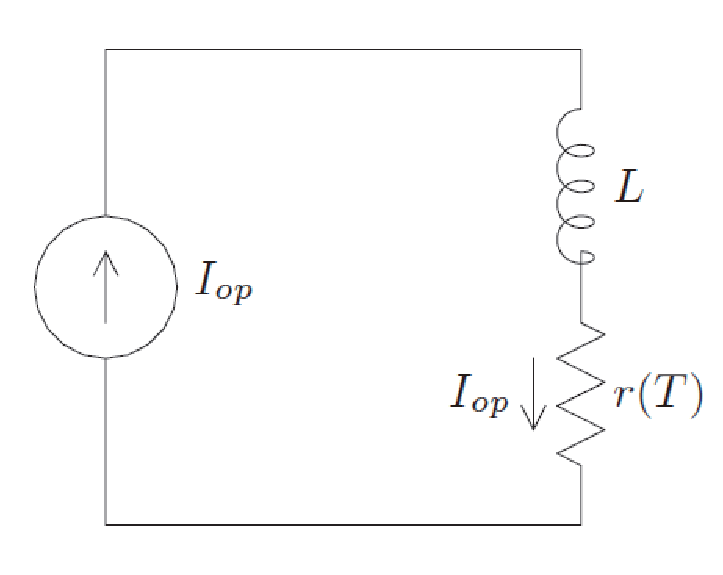
\includegraphics[scale=0.5]{chpt8/figs/fig8.1.eps}
	\caption{电路模型:电感为$L$的超导磁体,有依赖于温度的正常区电阻$r(T)$,连基于恒流$I_{op}$源。}
\end{figure}
图8.2给出了银(0$^\circ$C和4$^\circ$C的电阻率RRR=1000;100)、铜(200;100;50)、铝(级别:1000)和黄铜(70Cu-30Zn)的$Z(T,0)$。
虚线(不易看出)是$\tilde{\rho}_m=5.5\times 10^{-8}\Omega$m(方程8.10b)的黄铜。对任意的$T_i,T_f$组合,有:
\begin{equation}% 8.11
Z(T_f,T_i)=Z(T_f,0)-Z(T_i,0)=Z(T_f)-Z(T_i)
\end{equation}
对任意的$T_i,T_f$组合,存在一个加热时间$\tau_{ah}^i(T_f,T_I)$---
角标$i$表示恒电流加热---有下式给出:
\begin{equation}% 8.12a
\tau_{ah}^{i}(T_f,T_i)=\left(\frac{1+\gamma_{m/s}}{\gamma_{m/s}}\right)\frac{Z(T_f,T_i)}{J_{m_o}^{2}}
\end{equation}
类似的,对任意的$T_i,T_f$组合,在恒电流加热时间$\tau_{ah}$内存在一个基底电流密度$J_{m_o}^i(T_f,T_i)$:
\begin{align*}% 8.12b
J_{m_o}^{i}(T_f,T_i)=\sqrt{\left(\frac{1+\gamma_{m/s}}{\gamma_{m/s}}\right)\frac{Z(T_f,T_i)}{\tau_{ah}}} \tag{8.12b}
\end{align*}

因为在$\sim 300$ K以上,$C_m(T)$存在渐近线,而$\rho_m(T)$却继续随$T$增长。被积函数$C_m(T)/\rho_m(T)$随$T$减小,
所以$Z(T_f,T_i)$的很小增量会引起(多数实际损坏的)绕组$T_f$的剧烈增加:保持$T_f$不大于200 K。

\begin{figure}
	\centering
	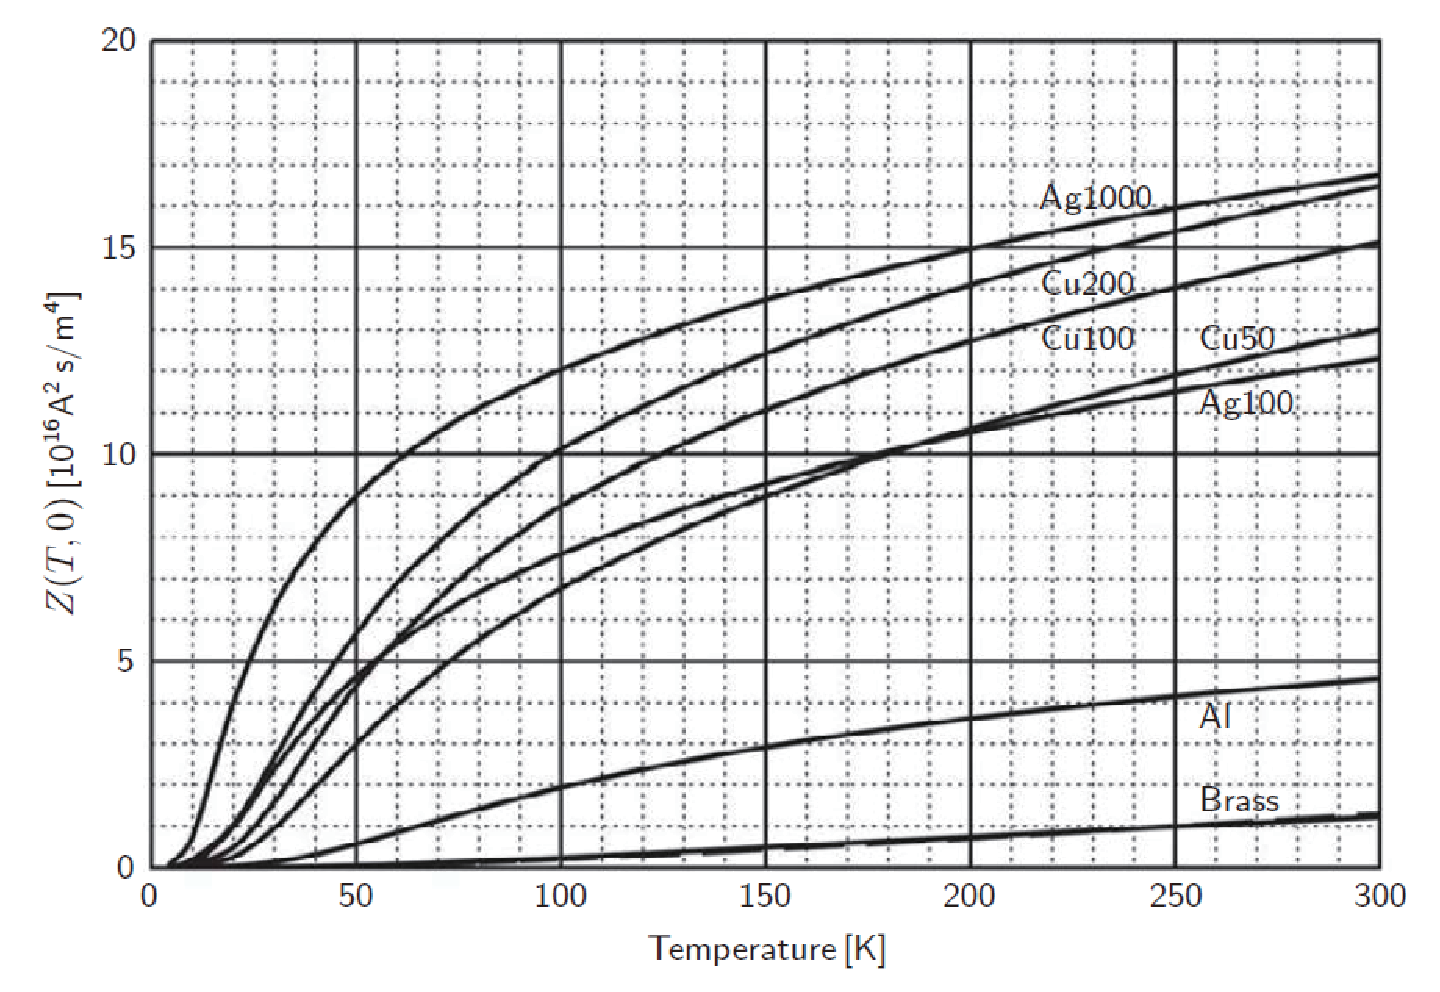
\includegraphics[scale=0.5]{chpt8/figs/fig8.2.eps}
	\caption{几种常用金属材料的$Z(T, 0)$图。}
\end{figure}

\subsection{放电模式下的绝热加热}
本节我们研究超导磁体($L$)中正常电阻区域$r(t)$---或$r(T)$---在放电模式下的绝热加热,
这种模式在超导磁体保护中经常遇到。
实际的例子在后面的专题中给出。

磁体最初($t=0$)由电流$I_{op}$供电,由泄流(放电)电阻($R_D$)将之旁路。
图8.3给出了电路图,其中,$I_m(t)$是时变基底金属电流。
$V_D\equiv R_d I_m(0)=R_d I_{op})$是$t=0$时刻放电电阻上的放电电压。

和方程8.9的绝热加热假设相同,但$J_{m_o}=I_{op}/A_m$(常数)由$J_m(t)\equiv I_m(t)/A_m$代替:
\begin{equation}% 8.13
C_m(T)\frac{dT}{dt}=\left(\frac{A_m}{A_{cd}}\right)\rho_m(T)J_{m}^{2}(t)
\end{equation}

$I_m(t)$的电路方程为:
\begin{equation}% 8.14
L\frac{dI_m(t)}{dt}+[R_D+r(t)]I_m(t)=0
\end{equation}

对多数情况,简化假设$R_D\gg r(t)$成立。方程8.14中解出$I_m(t)$。考虑到$\tau_{dg}=L/R_D$,可以得到$J_m(t)$:
\begin{equation}% 8.15
J_m(t)=J_{m_o}e^{-t/\tau_{dg}}
\end{equation}
式中,$J_{m_o}\equiv J_{m}(t=0)$。联立8.13和8.15,使用$Z(T_f,T_i)$的定义,有:
\begin{subequations}% 8.16a 8.16b 8.16c
	\begin{align}
Z(T_f,T_i)&=\left(\frac{A_m}{A_{cd}}\right)\int_{0}^{\infty}J_{m_o}^{2}e^{-2t/\tau_{dg}}dt=\left(\frac{A_m}{A_{cd}}\right)J_{m_o}^{2}\times\frac{1}{2}\tau_{dg} \\
&=\left(\frac{A_m}{A_{cd}}\right)J_{m_o}^{2}\left(\frac{L}{2R_D}\right)\\ 
&=\left(\frac{\gamma_{m/s}}{1+\gamma_{m/s}}\right)J_{m_o}^{2}\left(\frac{L}{2R_D}\right)
\end{align}
\end{subequations}

\begin{figure}
\centering
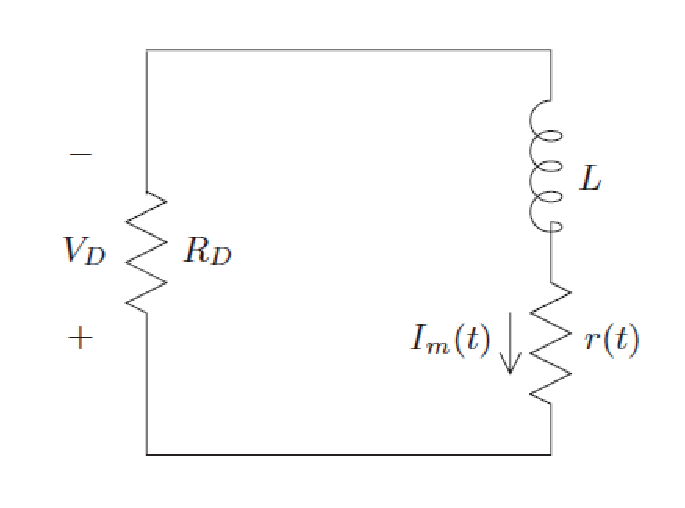
\includegraphics[scale=0.5]{chpt8/figs/fig8.3.eps}
\caption{电路模型:电感为$L$的超导磁体,有依赖于$T(t)$的正常区电阻$r(t)$,在放电模式下绝热加热。
	放电电阻$R_D$旁路磁体端子。$V_D\equiv R_d I_m(0)$是$t=0$时刻$R_D$上的放电电压}
\end{figure}

磁体电感$L$和放电电阻$R_D$可以分别由磁体初始存储磁能$E_m$和$R_D$上的初始放电电压$V_D$表示。即:
\begin{subequations}
	\begin{align}
	L&=\frac{2E_m}{I_{op}^{2}}\\
	R_D&=\frac{V_D}{I_{op}}
	\end{align}
\end{subequations}

联立8.16b,8.17a和8.17b,得到:
\begin{equation}% 8.18a
Z(T_f,T_i)=\left(\frac{A_m}{A_{cd}}\right)\frac{J_{m_o}^{2}E_m}{V_DI_{op}}
\end{equation}
该方程表明,$T_f$在大$J_{m_o}$和/或$E_m$以及小$V_D$和/或$I_{op}$的组合下较大。
我们可以考虑将比值$E_m/V_D I_{op}$作为有效放电时间,其中$V_D I_{op}$是有效放电功率。
由$J_{m_o}=I_{op}/A_m$,我们将8.18化简为:
\begin{align*}% 8.18b
Z(T_f,T_i)=\frac{J_{m_o}^{2}E_m}{A_{cd}V_D} \tag{8.18b}
\end{align*}

在放电模式下,对任意绕组温度极限$T_f$,存在一个最大的基底电流密度$J_{m_o}^D$:
\begin{equation}% 8.19
J_{m_o}^{D}=\frac{A_{cd}V_DZ(T_f,T_i)}{E_m}
\end{equation}

方程8.19给出了完全不同于6.22所给的低温稳定性判据的$J_{m_o}$判据。

\subsection{引线短接的磁体的绝热加热}
假设一个电感为$L$的磁体端子短接,在$t=0$时刻绕组中出现了一小块正常区域,如图8.4;
电流$I_m(t)$在电阻为$r(T)$的正常区基底金属流动。
\begin{figure}
	\centering
	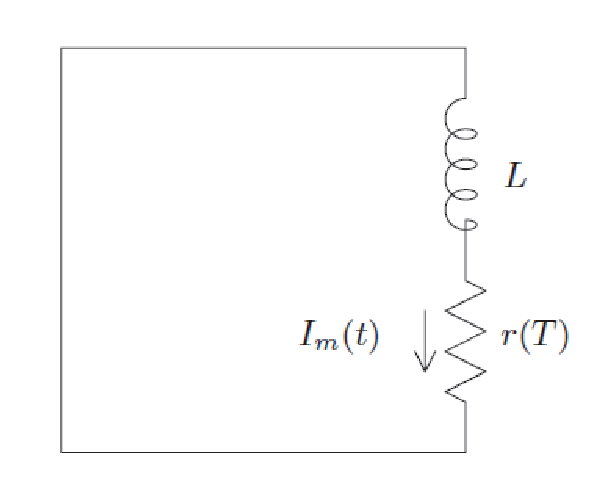
\includegraphics[scale=0.5]{chpt8/figs/fig8.4.eps}
	\caption{电路模型:电感为$L$的磁体端子短接,有依赖于温度的正常态区域电阻$r(T)$,绝热加热。
	正常态区域的电流为$I_m(t)$。}
\end{figure}

基底金属电流$I_m(t)$的控制方程为:
\begin{equation}% 8.20
L\frac{dI_m(t)}{dt}+r(T)I_m(t)=0
\end{equation}
温度依赖的$r(T)$显然随时间增加。有两个原因:1) 磁场能被转化为热能,使正常态区域温度升高;2)
正常态区域自身在绕组内扩散。
为了我们的分析,使用\textit{最简单}的假设:正常态区域电阻为常数,$r(T)=R_{nz}$:
\begin{equation}% 8.21
R_{nz}=\frac{\rho_m(T_f)\ell_{nz}}{4A_m}
\end{equation}
式中,$\rho_m(T_f)$是正常态最终温度下的基底电阻率;
$\ell_{nz}$是电流衰减到零时处于电阻态的总导体长度。
分母中的因子4来源于正常态区域温度$T_i$和$T_f$之间在空间(2)和时间(2)上的“平均”。
方程8.21同时假定了$\rho_m(T_f)\gg \rho_m(T_i)$,在一些特定的$T_i$和$T_f$组合下可能是不成立的,
但这个简化引入的不确定性相比8.21给出的基本假设引起的不确定性要小得多。
在$R_{nz}$时,$J_m(t)=I_m(t)/A_m$,由$J_m(t=0)=I_{op}/A_m=J_{m_o}$,得:
\begin{equation}% 8.22
J_m(t)=J_{m_o}e^{-t/(L/R_{nz})}
\end{equation}

在绝热加热时,我们得到:
\begin{subequations}% 8.23a,b,c
	\begin{align}
Z(T_f,T_i)&=\left(\frac{A_m}{A_{cd}}\right)\int_{0}^{\infty}J_{m_o}^{2}e^{-2t/(L/R_{nz})}dt\\
Z(T_f,T_i)&=\frac{1}{2}\left(\frac{A_m}{A_{cd}}\right)J_{m_o}^{2}\left(\frac{L}{R_{nz}}\right) \\
&=\frac{1}{2}\left(\frac{A_m}{A_{cd}}\right)J_{m_o}^{2}\tau_{dg}
\end{align}
\end{subequations}
式中,$\tau_{dg}=L/R_{nz}$是有效放电时间常数。
对一个参数为$a_1,\alpha$,总匝数为$N$的螺管线圈,驱动到正常态的总复合导体长度$\ell_{nz}$为:
\begin{equation}% 8.24
\ell_{nz}=f_r\pi a_1(\alpha+1)N
\end{equation}
式中,$f_r$是出于电阻态的绕组体积分数,与8.6同。
联立8.21和8.24,有:
\begin{equation}% 8.25
R_{nz}=f_r\frac{\rho_m(T_f)\pi a_1(\alpha+1)N}{4A_m}
\end{equation}

我们可以用$L$和其他磁体参数(方程3.81)表示$N$:
\begin{equation}% 8.26
N=\sqrt{\frac{L}{\mu_oa_1\ \mathcal{L}(\alpha,\beta)}}
\end{equation}

于是,$R_{nz}$可以写为:
\begin{equation}% 8.27
R_{nz}=f_r\frac{\pi(\alpha+1)\rho_m(T_f)}{4A_m}\sqrt{\frac{a_1L}{\mu_o\ \mathcal{L}(\alpha,\beta)}}
\end{equation}

这样,我们可以得到放电时间常数$\tau_{dg}$:
\begin{subequations}% 8.28a,b
	\begin{align}
\tau_{dg}&=\frac{L}{R_{nz}}=\frac{4A_m}{f_r\pi(\alpha+1)\rho_m(T_f)}\sqrt{\frac{\mu_o\ \mathcal{L}(\alpha,\beta)L}{a_1}}\\
\tau_{dg}&=\frac{4}{f_r\pi(\alpha+1)\rho_m(T_f)J_{m_o}}\sqrt{\frac{2\mu_o\ \mathcal{L}(\alpha,\beta)E_m}{a_1}}
\end{align}
\end{subequations}
式中,$J_{m_o}=I_{op}/A_m, L=2E_m/I_{op}^2$,其中$E_m$是磁体的初始磁场能储量。

联立8.23c和8.28b,有:
\begin{equation}% 8.29
\rho_m(T_f)Z(T_f,T_i)=\left(\frac{A_m}{A_{cd}}\right)\frac{2J_{m_o}}{f_r\pi(\alpha+1)}\sqrt{\frac{2\mu_o\ \mathcal{L}(\alpha,\beta)E_m}{a_1}}
\end{equation}

方程8.29中可以解出$T$。
如前面8.1.2所提及的,$T_f$严重依赖于$f_r$。对于8.1.2中的实例,为了在$B_o\ge 5$ T时确保$T_f$低于200 K,$f_r$至少$\sim 0.1$。
这个条件对具有小正常区传播(NZP)速度的HTS是很难满足的,8.4会继续讨论。

尽管$f_r$是未知的,但对一个给定的$T_f$和$T_i$组合,存在一个最大基底电流密度$J_{m_o}^{sh}$限制了短接磁体的过热:
\begin{subequations}% 8.30a,b
	\begin{align}
J_{m_o}^{sh}=\frac{1}{2}\left(\frac{A_{cd}}{A_m}\right)f_r\pi(\alpha+1)\rho_m(T_f)Z(T_f,T_i)\sqrt{\frac{a_1}{2\mu_o\ \mathcal{L}(\alpha,\beta)E_m}}\\
J_{m_o}^{sh}(T_f,T_i)=\frac{1}{2}\left(\frac{A_{cd}}{A_m}\right)\frac{f_r\pi(\alpha+1)\rho_m(T_f)Z(T_f,T_i)}{\mu_o\ \mathcal{L}(\alpha,\beta)NI_{op}}
\end{align}
\end{subequations}
b式是在a式中代入$E_m=\mu_o a_1\mathcal{L}(\alpha,\beta)N^2 I_{op}^2/2$得到的。
如我们所料,$J_{m_o}^{sh}$在大$f_r$和$T_f$以及小$E_m$组合下为增函数。
8.30b表明,大安匝数的螺管线圈必须在小$J_{m_o}^{sh}$下运行。


\subsection{恒定电压模式下的绝热加热}
最后,考虑一个超导磁体,整个绕组全部为电阻性,导体总长度为$\ell_{cd}$,电阻为$R_m(T)$,连接于恒定电压源,如图8.5所示。
这里,整个绕组的温度为$T(t)$。
考虑$R_m(T)=\rho_m(T)\ell_{cd}/A_m$,功率密度方程类似于8.9a:
\begin{subequations}% 8.31a,b
	\begin{align}
A_{cd}\ell_{cd}C_{cd}(T)\frac{dT}{dt}&=\frac{V_{op}^{2}}{R_n(T)}=\frac{V_{op}^{2}A_m}{\rho_m(T)\ell_{cd}}
C_m(T)\frac{dT}{dt}\\
&\simeq\left(\frac{A_m}{A_{cd}}\right)\frac{V_{op}^{2}}{\rho_m(T)\ell_{cd}^{2}}\\
\int_{T_i}^{T_f}C_m(T)\rho_m(T)dT&=\left(\frac{A_m}{A_{cd}}\right)\frac{V_{op}^{2}}{\ell_{cd}^{2}}\tau_{ah}
\end{align}
\end{subequations}
式中,$\tau_{ah}$是在恒定电压模式下的加热时间。
根据$Z(T_f,T_i)$,我们可以定义函数$Y(T_f,T_i)$。类似于8.10b,可以针对合金基底金属作简化。类似于$Z(T_f,T_i)$,$Y(T_f,T_i)$
也可以写成两个单一温度的函数。
\begin{subequations}% 8.32a,b,c
	\begin{align}
Y(T_f,T_i)&\equiv\int_{T_i}^{T_f}C_m(T)\rho_m(T)dT\\
Y(T_f,T_i)&\simeq\tilde{\rho}_m[H_m(T_f)-H_m(T_i)]\\
Y(T_f,T_i)&=Y(T_f)-Y(T_i)
\end{align}
\end{subequations}

图8.6给出了$Y(T,0)$图,该图中的金属和图8.2中的$Z(T,0)$所对应的相同。
金属的纯度,通常在$\sim$50 K之下对$\rho_m$影响很大。
于是,纯度对$Z(T,0)$想想很大,而对$T>\sim$100 K时的$Y(T,0)$影响很小。

类似于8.9c,我们从8.31b可以导出:
\begin{equation}% 8.33
Y(T_f,T_i)=\left(\frac{A_m}{A_{cd}}\right)\frac{V_{op}^{2}\tau_{ah}}{\ell_{cd}^{2}}
\end{equation}
\begin{figure}
	\centering
	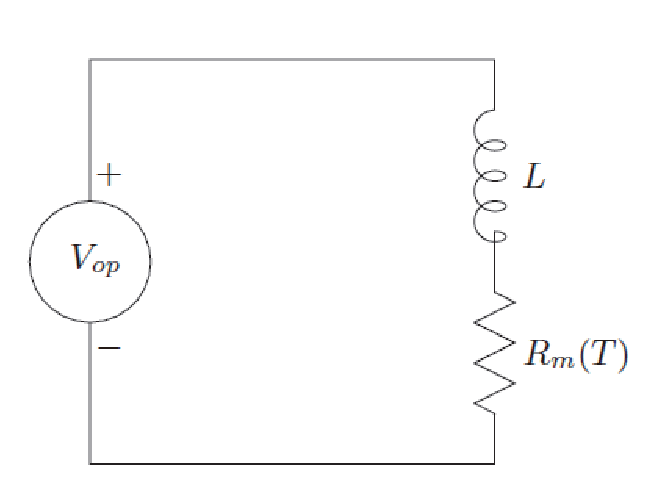
\includegraphics[scale=0.5]{chpt8/figs/fig8.5.eps}
	\caption{电路模型:电感为$L$的超导磁体,全部绕组处于正常态,电阻为$R_m(T)$,在恒压源加热模式。}
\end{figure}

注意到螺管线圈在$f_r=1$的$\ell_{cd}$已由8.24给出,使用8.26,我们得到:
\begin{equation}% 8.34
\ell_{cd}=\pi(\alpha+1)\sqrt{\frac{a_1L}{\mu_o\ \mathcal{L}(\alpha,\beta)}}
\end{equation}

将8.34中的$\ell_{cd}$代入8.33,有:
\begin{equation}% 8.35
Y(T_f,T_i)=\left(\frac{A_m}{A_{cd}}\right)\frac{\mu_o\ \mathcal{L}(\alpha,\beta)V_{op}^{2}\tau_{ah}}{\pi^2(\alpha+1)^2a_1L}
\end{equation}

对任意$T_f$和$T_i$组合,在恒压加热模式下,存在一个加热时间极限$\tau_{ah}^v$:
\begin{equation}% 8.36
\tau_{ah}^{\upsilon}=\left(\frac{A_{cd}}{A_m}\right)\frac{\pi^2(\alpha+1)^2a_1L}{\mu_o\ \mathcal{L}(\alpha,\beta)}\left[\frac{Y(T_f,T_i)}{V_{op}^{2}}\right]
\end{equation}

因为$\rho_m(T)$随温度$T$增加,$Y(T,0)$在$T$超过300 K之后继续增加。
因为超导磁体处于正常态的总电阻$R_m(T)$正比于$\rho_m(T)\ell_{cd}$,
通过磁体的加热电流由$V_{op}/R_m(T)$给出,它随$T$增加而减小。
这意味着$\tau_{ah}^v$比$T_f$增加的更快;也即在恒压加热模式下,比在恒流模式下更不容易热失控。
因此,就加热超导磁体而言,恒压模式要比恒流模式更安全。本问题将在问题8.1中进一步研究。

\begin{figure}
	\centering
	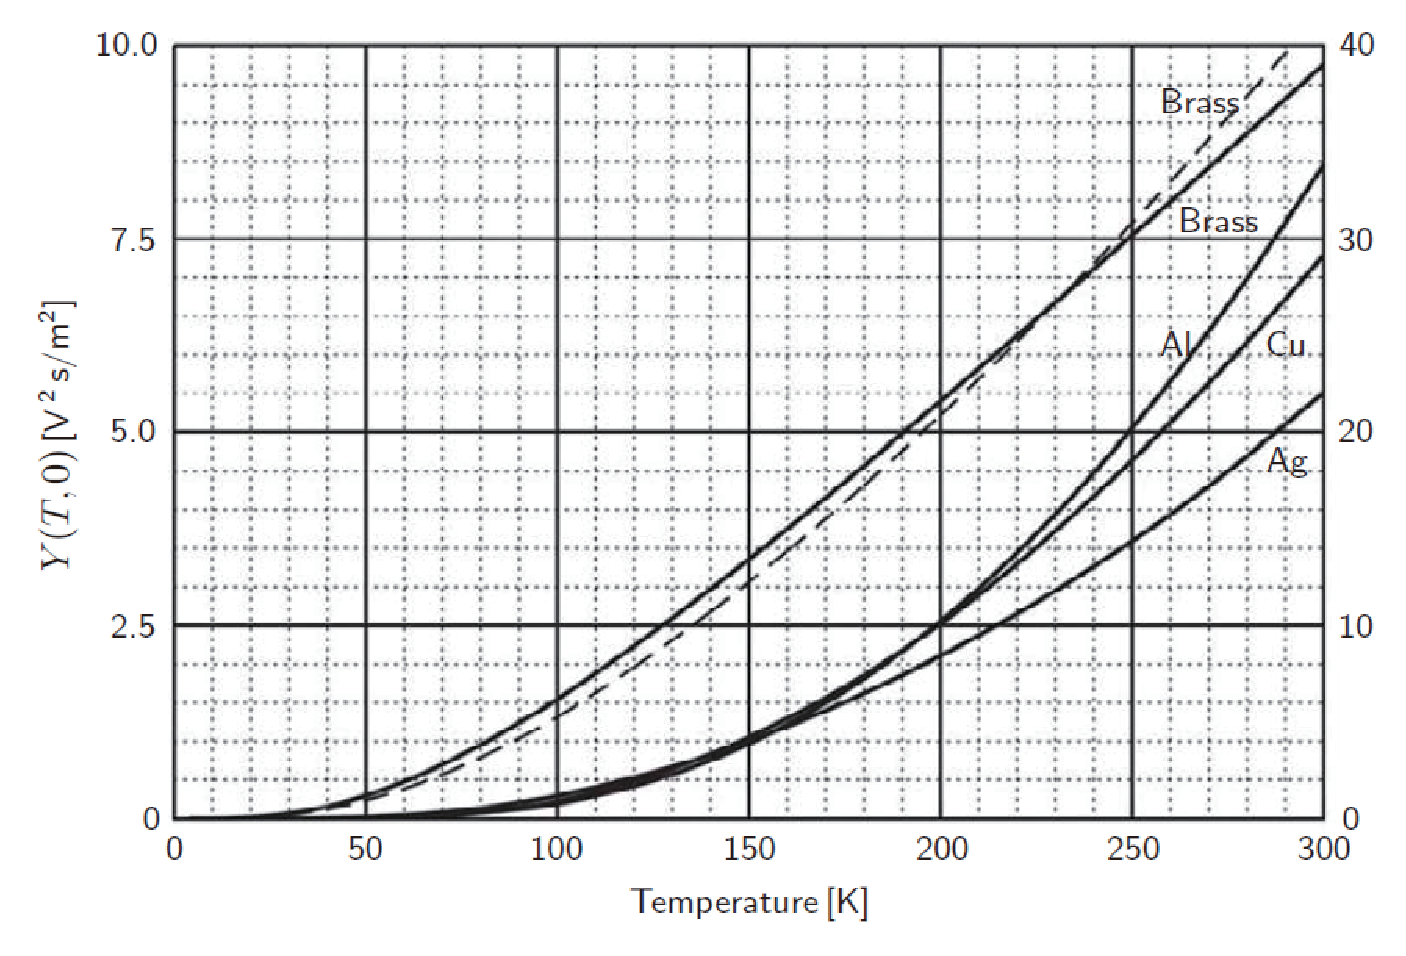
\includegraphics[scale=0.5]{chpt8/figs/fig8.6.eps}
	\caption{$Y(T,0)$图。左侧纵轴是Ag、Cu、Al的刻度,右侧纵轴是黄铜的刻度。
	在温度超过约100 K后,$Y(T,0)$几乎与Ag和Cu的纯度无关。}
\end{figure}



\section{高电压}
大多数超导磁体的一个吸引人的特征是励磁所需的“低”电压,即$\sim$10 V。对于产生相同场强的普通金属磁体该值$>100$ V。
磁体运行包括三个时间区间:1)充电励磁; 2)恒定磁场静态运行; 3)放电去磁。 
不幸的是,这种低电压充足性通常仅在前两个时间区间可以保证;
区间3可能遇到非常高的电压,特别是它处于故障模式的时候。
 当然,由于磁体失超,在区间1和区间2期间可能会突然进入区间3。
 由于超导磁体是电感器,其端电压包含一个电感分量,由下式给出:
 \begin{align}
V=L\frac{dI}{dt}
 \end{align}
注意到$L=2E_m/I_o^2$,其中$I_o$是区间3开始时的磁体电流。
因为在这个区间,磁体电流下降$\Delta I$通常等于$I_o$,我们可以将8.37改写为:
\begin{align*}
V=\frac{2E_m}{I_{o}^{2}}\left(\frac{\Delta I}{\Delta t}\right)\approx\frac{2E_m}{I_o\Delta t}\tag{8.37b}
\end{align*}

保护主要在那些$E_m$超过$\sim$ 100 kJ的磁体才非常关键;
储能量小于这个级别的磁体是可以补救的,或者至少不会引起严重的困难。
如果我们设定实际超导磁体的危险电压等级是1 kV,那么根据8.37b,
在$E_m=100$ kJ时,任意小于200 As的$I_o\Delta t$组合值都会产生高于1 kV
的电压,磁体中的能量将足以引起严重破坏。
一个实例:运行于$I_o=1$ kA的100 kJ磁体,如果电流在$\sim$200 ms级别放电。
随着储能量的增加,问题越来越严重[8.17]。

根据8.37b,我们还可以看到,电流引线必须承受较高的放电电压。
Anishchenko、Heller等[8.18]和Gerhold[8.19]已开发出可以承受高压的电流引线。

\subsection{电弧环境}
超导绕组可能工作于一个设计者可以选择的环境中,比如1) 真空 vs. 非真空;2) 液体 vs. 气体;和/或 3) 氦 vs. 氮。
在防止电弧方面,除了在Paschen压力附近,真空要优于非真空;液体优于气体;氮优于氦.
不过,放电可能会破坏设计者的环境选择。
故障引起的绕组加热会破坏设计条件:1)它可能加快系统排气,使系统维持高真空变得困难;或者2)它可能将局部的环境从液体变为气体。

自1970年代初,人们开始归集制冷工质的绝缘击穿数据[8.20,8.21]。
Gerhold给出了氮和氦的击穿数据[8.22]。
在超导磁体中,存在很多影响电弧的设计项目,尚无普适的明确数据。
Schultz简明的探讨了这个大问题,给出了不少图表和数据[1.28,8.11]。

表8.4.。。。。。。。。。。。。。。。

\subsection{Paschen电压试验}
表8.4给出了\textit{室温}气体的最小电弧放电电压$V_{mn}$以及对应的$Pd$数据。
$P$是气体压力,$d$是施加电压$V_{mn}$的电极距离。
注意到双原子分子的$V_{mn}$要比惰性气体的搞。

Paschen电压试验是放电电压超过1 kV的超导磁体的例行试验。
低温容器试验时,将电流引线和测试电缆连接于高压,将低温容器抽空至某压力(如$P\sim 10^{-3}$ torr)之下。
如果在电压升高至$V_{mn}$期间没有泄漏电流,则在下一个压力水平下(从$P\sim 10^{-2}$ torr到大气压)重复上述试验。
系统在进行更复杂的高压测试前,必须通过如上简单的试验。

\subsection{失超磁体内的电压峰值}
使用一个简单的模型,引入额外的简化假设,我们研究失超超导磁体在其端子短接时的内部电压峰值[1.27;8.25]。
在以下两种超导磁体模式下,端子短接工况在一个很短的时间内很可能出现:
1) 在区间1,当磁体连接于恒压电流源,磁体电流增至进入它的区间2;
2) 当区间2的磁体被持续模式开关旁路。
任一模式下,当故障迫使(主动保护)或自动(被动保护)地令超导磁体进入区域3,端子不能在被视为短接。
不过,在这个时候,特别是当磁体是主动保护的时候,因为转移的延迟,损坏可能已经发生。

\textbf{内部电压分布}

在一个内部正常区扩散的旁路磁体中,内部电压的分布与绕组内的正常区分布有关。
图8.7给出了磁体内的电压分布,其中绕组从接地的端子绕向另一个接地的端子。
单位导体长度的电感假定为常数。
在8.7a中,10\%($f_r=0.1$)的绕组从一个端子开始,已经进入电阻态;
在8.7b中是20\%;在8.7c中是50\%;在8.7d中是100\%。

\begin{figure}
	\centering
	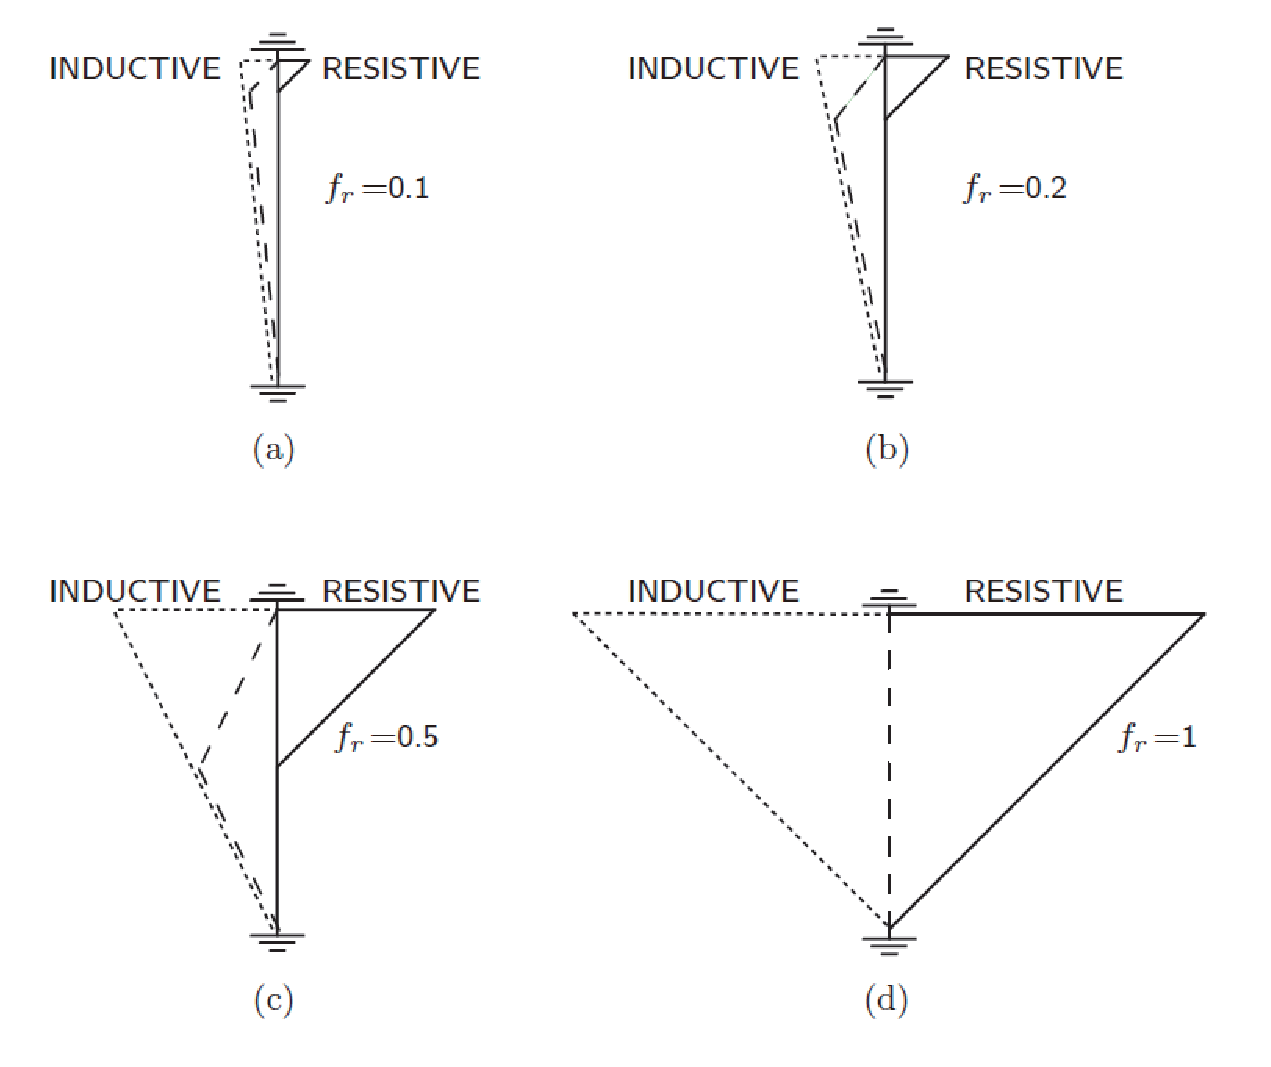
\includegraphics[scale=0.5]{chpt8/figs/fig8.7.eps}
	\caption{电压分布。}
\end{figure}

在图8.7的每一组电压分布中,实线表示阻性电压;短虚线表示感性电压;长虚线表示作为电阻性和点感性电压之和的总内部电压。
每一个图中,磁体电流保持恒定为$I_{op}$。
实际中,电流似乎随时间减小的;这个减小的效应在后面将会考虑。

最高阻性电压$[V_r]_{mx}$发生在磁体的一个端子上。因为端子是接地的,它恰好与同等复制的感性电压$[V_r]_{mx}=R_{nx}I_{op}$匹配,
其中$R_{nx}$是总的正常态电阻,如方程8.25所给。

从图8.7中我们得到最大内部电压为:
\begin{equation}% 8.38
[V_{in}]_{mx}=f_r(1-f_r)R_{nz}I_{op}
\end{equation}
其中,$f_r$如方程8.6已指出的,是被驱至电阻态的绕组体积分数。
注意到磁体电流维持$I_{op}$。
方程8.38表明在$f_r\rightarrow 0$或$f_r\rightarrow 1$时有$[V_{in}]_{mx}\rightarrow 0$。
方程还表明$[V_{in}]_{mx}$的峰值出现在$f_r=0.5$。

联立8.25和8.38,有:
\begin{equation}% 8.39
[V_{in}]_{mx}=f_r(1-f_r)\frac{\pi(\alpha+1)\rho_m(T_f)a_1}{4A_m}NI_{op}
\end{equation}

\textbf{基底电流密度的电压判据}

最大内部电压出现的条件为:正常区扩散到占绕组的$50\%$而电流仍维持$I_{op}$;或初始时绕组即有50\%被驱至正常态。

我们可以得到限制带旁路螺管磁体内部感应电压不超过击穿值$V_{bk}$的基底电流密度$J_{m_o}^V$的表达式:
\begin{equation}% 8.40a
J_{m_o}^{V}=\frac{2}{f_r(1-f_r)}\left[\frac{F(\alpha,\beta)}{\pi(\alpha^2-1)\beta}\right]\left[\frac{\mu_oV_{bk}I_{op}}{a_{1}^{2}\rho_m(T_f)B_o}\right]
\end{equation}
类似的,我们可以得到一个直接看出与$E_m$依赖关系的表达式:
\begin{align*}% 8.40b
J_{m_o}^{V}=\frac{2}{f_r(1-f_r)}\left[\frac{\sqrt{\ \mathcal{L}(\alpha,\beta)}}{\pi(\alpha+1)}\right]\left[\frac{V_{bk}I_{op}}{\rho_m(T_f)}\sqrt{\frac{2\mu_o}{a_1E_m}}\right] \tag{8.40b}
\end{align*}

可以看到,$J_{m_o}^V$随$V_{bk}$和$I_{op}$的乘积增长。
这里最重要的是,$J_{m_o}^V$随正常态金属的电导率增大而提高。
此外,一个较大的$V_{bk}$意味着较大的$J_{m_o}^V$,但是$I_{op}$下的绕组的电流密度$\lambda J_{op}$(6.3.3)
因为需要更多绝缘会很小。

\section{正常区传播(NZP)}
为了保护,多数“实际”大小的HTS磁体都必须依赖于一类或另一类主动技术,其中的一些将在后文讨论。
不过,对任何主动保护技术,因为在非恢复正常区的检测和电流退降之间存在不可避免的延迟,所以令磁体的正常区域传播(NZP)
速度“加快”,进而扩大其$f_r$(它限制$e_{mr}$(方程8.7),加强$J_{m_o}^{sh}$(方程8.30)和$J_{m_o}^V$(方程8.40))就很重要了。
一个具有快NZP速度(三个方向)的磁体可以成为“自保护”的;
自保护磁体的更多细节后文将讨论。
因为NZP速度在HTS绕组中通常比在LTS绕组中慢很多,故“自保护”HTS磁体几乎不可能实现:
\textit{所有}的HTS磁体都需要主动保护。

\subsection{轴向NZP速度}
自1960年代以来,LTS和HTS测试样品、模型绕组和磁体在绝热、准绝热、冷却条件下的长度方向
(沿着导体轴向)的NZP速度$U_\ell$得到了全面的研究[8.1, 8.2, 8.25–8.75]。
它是高性能(绝热)磁体保护的重要参数之一。
在那些绝热或准绝热的绕组中,NZP不仅限于导体轴向,而是三维扩散的:$U_t\propto U_\ell$,
其中$U_t$是“横向”传播速度。

\subsubsection*{绝热条件下的NZP}
图8.8给出了绝热条件下载流为$I$的导体示意图,正常-超导边界在$x=0$处,边界以恒定速度$U_\ell$沿$+x$方向移动。
正常态超导体的功率密度方程由不含扰动和冷却项的方程6.1的一维($x$)形式给出:
\begin{equation}% 8.41a
C_n(T)\frac{\partial T_n}{\partial t}=\frac{\partial}{\partial x}\left[k_n(T)\frac{\partial T_n}{\partial x}\right]+\rho_n(T)J^2
\end{equation}
其中,$C_n(T),k_n(T)$和$\rho_n(T)$分别是正常态超导体的热容、热导率和电阻率。

\begin{figure}
	\centering
	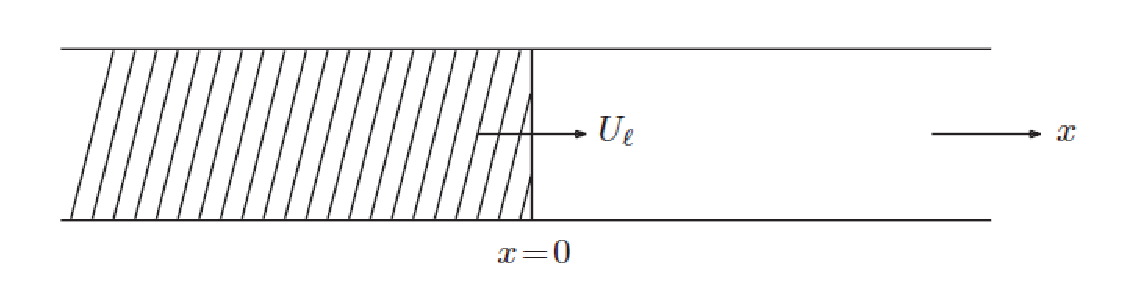
\includegraphics[scale=0.6]{chpt8/figs/fig8.8.eps}
	\caption{一维正常-超导边界($x=0$)以恒定速度$U_\ell$沿长度方向(轴向)移动。阴影部分($x<0$)
		为正常态区域,右侧为超导区域。}
\end{figure}

类似的,超导区域在绝热条件下的$x$方向的功率密度方程为:
\begin{align*}% 8.41b
C_s(T)\frac{\partial T_s}{\partial t}=\frac{\partial}{\partial x}\left[k_s(T)\frac{\partial T_s}{\partial x}\right] \tag{8.41b}
\end{align*}
其中,$C_s(T),k_s(T)$是超导态的热容和热导率。
当正常-超导边界在$+x$方向以恒定速度$U_\ell$移动时,我们可以将$x$坐标变换为$z$坐标:$z=x-U_\ell t$。
$\partial T_n/\partial t$可以写为:
\begin{equation}% 8.42
\frac{\partial T_n}{\partial t}=\frac{\partial T}{\partial z}\frac{\partial z}{\partial t}=-U_\ell\frac{dT}{dz}
\end{equation}

于是,我们可以吧8.41写成:
\begin{subequations}
	\begin{align}
-C_n(T)U_\ell\frac{dT_n}{dz}=&\frac{d}{dz}\left[k_n(T)\frac{dT_n}{dz}\right]+\rho_n(T)J^2\\
-C_s(T)U_\ell\frac{dT_s}{dz}=&\frac{d}{dz}\left[k_s(T)\frac{dT_s}{dz}\right]
	\end{align}
\end{subequations}
整理8.43a和8.43b,我们得到超导体分别在超导区($z>0$)和正常区($z<0$)的能量密度方程:
\begin{subequations}
	\begin{align}
&(z<0)\quad      \frac{d}{dz}\left[k_n(T)\frac{dT_n}{dz}\right]+C_n(T)U_\ell\frac{dT_n}{dz}+\rho_n(T)J^2&=0\\
&(z>0)\quad      \frac{d}{dz}\left[k_s(T)\frac{dT_s}{dz}\right]+C_s(T)U_\ell\frac{dT_s}{dz}&=0
	\end{align}
\end{subequations}
令$C_n(T),k_n(T), C_s(T)$和$k_s(T)$均为常数,分别记为$C_n,k_n, C_s$和$k_s$。假设$d^2 T_n/dz^2\simeq 0$,
我们可以重写8.44:
\begin{subequations}
	\begin{align}
	&(z<0)\quad     C_nU_\ell\frac{dT_n}{dz}+\rho_nJ^2&=0\\
&	(z>0)\quad     k_s\frac{d^2T_s}{dz^2}+C_sU_\ell\frac{dT_s}{dz}&=0
	\end{align}
\end{subequations}

从8.45b中可以直接解出$T_s(z)$:
\begin{equation}% 8.46a
T_s(z)=Ae^{-cz}+T_{op}
\end{equation}
式中,$T_{op}$是远离$z=0$($z\gg 0$)处的运行温度,
$c=C_s U_\ell/k_s$。
我们还知道$z=0$时由$T_s=T_t$,其中$T_t$是载流为$I$的超导体的转变温度。于是:
\begin{align*}% 8.46b
T_s(z)=(T_t-T_{op})\exp\left(-\frac{C_sU_\ell}{k_s}z\right)+T_{op} \tag{8.46b}
\end{align*}

另一个边界条件是各区域的$k(dT/dz)$应该在$z=0$处相等---
热流必须在边界上连续:
\begin{equation}% 8.47a
k_n\frac{dT_n}{dz}\mid_0=k_s\frac{dT_s}{dz}\mid_0
\end{equation}
联立8.45a,8.46b和8.47a,有:
\begin{align*}% 8.47b
-\frac{k_n\rho_nJ^2}{C_nU_\ell}=-C_sU_\ell(T_t-T_{op}) \tag{8.47b}
\end{align*}
在8.47b中解出$U_\ell$,有:
\begin{equation}% 8.48
U_\ell=J\sqrt{\frac{\rho_nk_n}{C_nC_s(T_t-T_{op})}}
\end{equation}

方程8.48中重要的几点包括$U_\ell$直接正比于电流密度$J$,而反比于两个区域热容的几何平均$\sqrt{C_n C_s}$。
8.48给出的$U_\ell$对绝热条件下的裸超导体有效。
由于材料物性是温度依赖的,使用$U_\ell$的精确表达式没什么必要。不过出于完整性,我们给出下面的精确表达式[8.47]:
\begin{equation}% 8.49
U_\ell=J\sqrt{\frac{\rho_n(T_t)k_n(T_t)}{\left[C_n(T_t)-\frac{1}{k_n(T_t)}\frac{dk_n}{dT}\mid_{T_t}\int_{T_{op}}^{T_t}C_s(T)dT\right]\int_{T_{op}}^{T_t}C_s(T)dT}}
\end{equation}

方程8.49给出的$U_\ell$值与YBCO带材短样在45-77 K的实测值吻合很好[8.66]。

取材料物性为常数,我们发现8.49退化为8.48。
在$C_n=C_s=C_o$时,方程8.48可以写为:
\begin{equation}% 8.50a
U_\ell=\frac{J}{C_o}\sqrt{\frac{\rho_nk_n}{(T_t-T_{op})}}
\end{equation}
在$(T_t-T_{op})/T_{op}\ll 1$时(一个通常可用于LTS而不能用于HTS的条件),我们可以修正8.50a,让它包含
温度依赖的$C_o,\rho_n$和$k_n$:
\begin{align*}% 8.50b
U_\ell=\frac{J}{C_o(\tilde{T})}\sqrt{\frac{\rho_n(\tilde{T})k_n(\tilde{T})}{(T_t-T_{op})}} \tag{8.50b}
\end{align*}
式中,$\tilde{T}=(T_t+T_{op})/2$。
方程8.48到8.50对没有基底金属的超导体有效;
实际中,磁体级导体都是复合的,我们可以用基底金属材料的物性近似上述材料属性。

\subsubsection*{复合超导体}
对于有截面为$A_m$的基底金属的复合导体,在$(T_t-T_{op})/T_{op}\ll 1$时(同样,只适用于LTS),
引入温度依赖的参数,利用$\tilde{T}=(T_t+T_{op})/2$,将8.50b推广为:
\begin{equation}% 8.51a
U_\ell=\frac{J_m}{C_{cd}}(\tilde{T})\sqrt{\frac{\rho_m(\tilde{T})k_m(\tilde{T})}{T_t-T_{op}}}
\end{equation}
式中,$C_{cd}(\tilde{T})$是导体在$T_{op}$和$T_t$区间的单位体积平均热容,
$J_m$是基底金属截面上的电流密度。
因为$\rho_m$(基底金属电阻率)远小于$\rho_n$,
$k_m$(基底金属热导率)远大于$k_n$,
8.51a中使用$k_m(\tilde{T})$和$\rho_m(\tilde{T})$是非常合适的。
方程8.51a中,Joshi建议转变温度$T_t\equiv (T_{cs}+T_{c})/2$[8.45],或简单的$T_t= (T_{cs}$。
试验数据很难验证这个微小的差异。
基于和方程8.9b相同的近似方法,我们使用$C_{cd}(\tilde{T})\simeq C_m(\tilde{T})$,有:
\begin{align*}% 8.51b
U_\ell\simeq\frac{J_m}{C_m}(\tilde{T})\sqrt{\frac{\rho_m(\tilde{T})k_m(\tilde{T})}{T_t-T_{op}}} \tag{8.51b}
\end{align*}

方程8.48-8.51的一般适用性已被大量LTS和最近的HTS试验证实。

\subsubsection*{长度方向NZP速度的实验确定}
确定$U_\ell$的实验基本装置很简单。
一般的,如图8.9所示,在一个长直样品上,测量很多短距离(10-20 cm)的局部电压信号;
在一些实验中,还监测了局部的温度。
如果测试样品处于磁体室温孔中,样品更倾向于环形或螺旋形而非平直的。
测试样品载流$I$时,由加热器等制造一个局部失超区域。
其过程通过电压信号$V_1,V_2,V_3$以及$V_\Sigma =V_1+V_2+V_3$监测;
明显,$U_\ell$可以从相邻电压(和/或温度)信号间距以及时间获得。
图8.9b给出了一段10 cm长Nb3Sn带的$V_1,V_2,V_3$以及$V_\Sigma =V_1+V_2+V_3$的记录波形[8.55]。

\begin{figure}
	\centering
	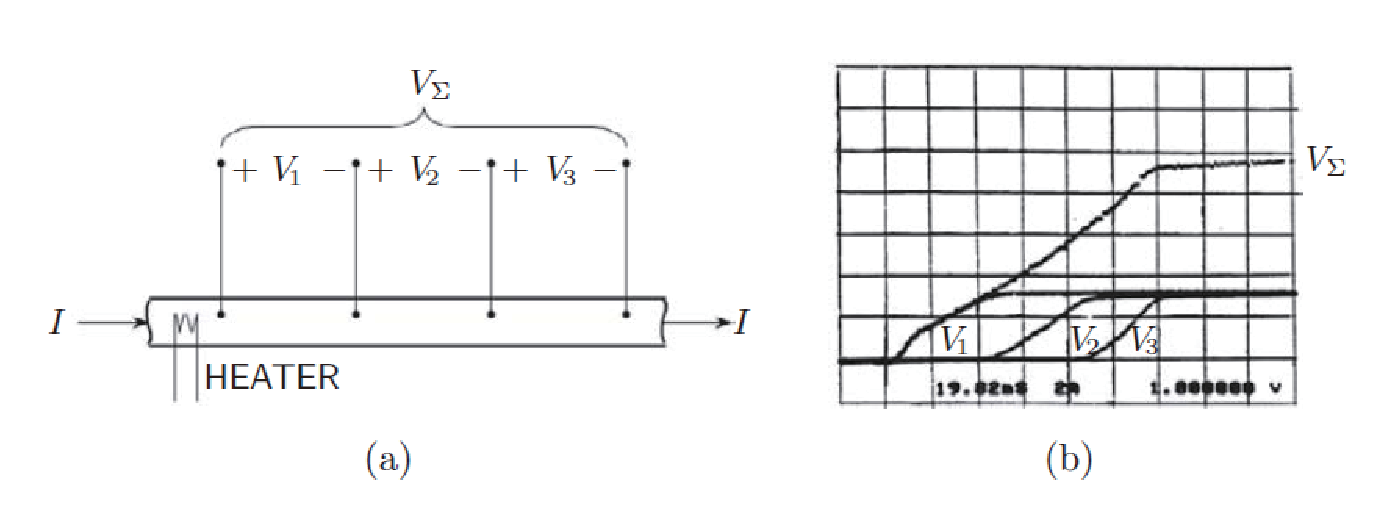
\includegraphics[scale=0.5]{chpt8/figs/fig8.9.eps}
	\caption{(a) 测量长度方向NZP速度的实验装置示意图;
		(b) NZP时间下的电压记录波形图。}
\end{figure}

使用类似于LTS测试所用的实验技术,在20实际初测量了上面描述的一个样品。
这里,不涉及实验设置的细节,我们仅在图8.10给出YBCO带材NZP速度测量的电压和温度的共四组曲线:
a),b)和c)是测试样品长度分别为20 cm[8.65],15 cm[8.70]和18 cm[8.74]情况下的$V(t)$曲线。
在20 cm场YBCO带材中,初始温度为50 K的样品的局部正常区域的产生依赖于在20 cm长度上的临界电流的非均匀分布。
72 A的过流脉冲(图8.10a和8.10d)触发了区域5的失超(相应的,$V_5$和$T_5$),导致恒定电流为30 A的NZP(图8.10a);
a)中的$V(t)$的时间刻度和d)中$T(t)$的时间刻度是一致的。
b)中的$V(t)$曲线是15 cm长带材在60 K的;c)中的是在70 K的。
测到的NZP速度在2-10 mm/s之间,总结如表8.5。

\begin{figure}
	\centering
	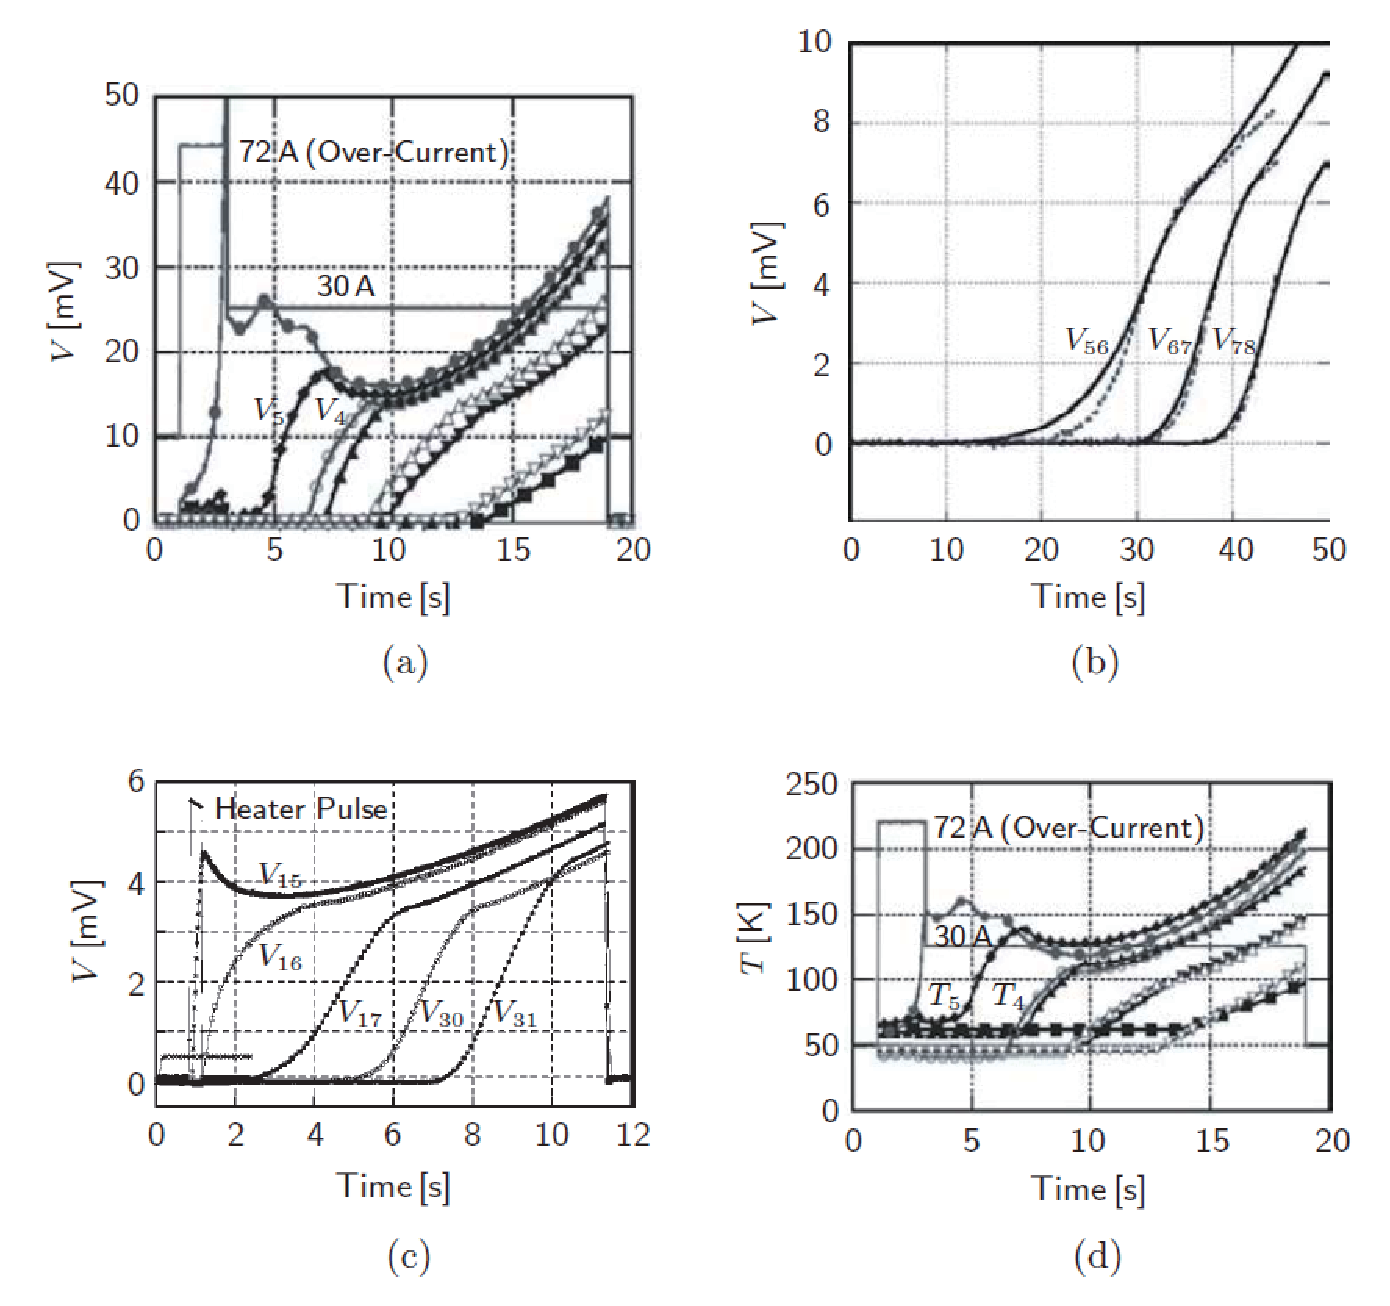
\includegraphics[scale=0.5]{chpt8/figs/fig8.10.eps}
	\caption{YBCO测试样品在长度方向的NZP信号。}
\end{figure}

表8.5.。。。。。。。。。。。。。。。。

表8.5列出了LTS和HTS的$U_\ell$测量值。
尽管由液氦冷却,Nb-Zr单丝的$U_\ell\propto J$,因为没有基底金属(Stekly之前时代的超导体),
正常态焦耳热完全超过了冷量。
一般的,这些数据表明HTS(Bi2223-Ag;YBCO)的NZP速度比LTS的小2-4个数量级。
NbTi的“恢复”[8.36]将在8.4.2讨论。
铁基底的MgB2[8.70],NZP速度和LTS的具有可比性,主要因为没有高导电基底金属。
这里,在总导体电流密度$J_{cd}$为$26\ \mathrm{ A/mm^2}$或更低时,
不会发生NZP:正常态超导体不产生足够的焦耳热,主要原因是其指数很低($n\simeq 15$)。
类似的非NZP行为在Bi2223-Ag[8.55]带和YBCO带[8.64,8.69,8.73]中都观察到了。

\subsection{“制冷”条件下的NZP}
尽管在冷却磁体中的NZP保护不及绝热磁体中那么重要,
但在有冷却条件下的NZP也获得了广泛的研究。
如表8.5中给出NbTi复合导体中观察到的,实际上存在一个“恢复”电流,低于
这个电流,正常态会缩小而不是扩大。

\subsection{横向(匝间)速度}
现在我们关注主要针对超导带材的横向(匝间)NZP速度$U_t$。
$\mathrm{Nb_3Sn}$带材曾一度很流行,但现在已不再用。
现在最广泛使用的复合超导体带材是HTS的Bi2223-Ag和YBCO,两者都可绕成饼式线圈。
此类HTS磁体的绕组尽管由制冷工质或制冷机冷却,但本质上是绝热的。
$U_\ell$的绝热分析可以用于导出$U_t$[8.57]:
\begin{equation}% 8.52
U_t=U_\ell\sqrt{\frac{1}{2}\left(\frac{\delta_{cd}}{\delta_i}\right)\left[\frac{k_i(\tilde{T})}{k_m(\tilde{T})}\right]}
\end{equation}
式中,$k_i(\tilde{T})$是相邻厚度为$\delta_{cd}$超导带之间的厚度为$\delta_i$的绝缘层的温度平均热导率。
方程8.52中,一般$\delta_{cd}>\delta_i$,倍数通常在3-10之间,但是$k_m\gg k_i$的倍数在1000或更大,
甚至在77 K时也是如此;所以,$U_t$至少比$U_\ell$小1到2个数量级。
Bi2223-Ag和YBCO模型线圈的测试实际上已经表明$U_t$至少比$U_\ell$小一个数量级。
因为有高导电基底的HTS的$U_\ell$本身仅为1-10 mm/s,$U_t$则更小。
如下面将讨论的,在2D和3D绕组中,接触热阻能进一步降低有效$U_t$。

\subsubsection*{接触热阻}
因为$U_t\propto \sqrt{k_i}$,使用高热导材料做匝间绝缘可以提高$U_t$。
一种这样的材料是钻石;液氮温区中钻石的体热导率是铜的10-100倍[8.54]。
不过,方程8.52忽略了导体和绝缘体之间的接触热阻。
实际上,由绝缘垫片隔开的相邻导体之间存在两个接触热阻$R_{th_{ct}^1}$和$R_{th_{ct}^2}$。
于是,方程8.52中的$k_i$应被$k_i^\prime$替换:
\begin{equation}% 8.53
\frac{1}{k_{i}^{\prime}}=\frac{1}{k_i}+R_{th_{ct}^{1}}+R_{th_{ct}^{2}}
\end{equation}

使用8.53中的$k_i^\prime$代入8.52,得到:
\begin{equation}% 8.54
U_t=U_\ell\sqrt{\frac{1}{2}\left(\frac{\delta_{cd}}{\delta_i}\right)\frac{k_i}{k_m[1+k_i(R_{th_{ct}^{1}}+R_{th_{ct}^{2}})]}}
\end{equation}

方程8.54表明当接触热阻是主要项,即$k_i(R_{th_{ct}^{1}}+R_{th_{ct}^{2}})\gg 1$时,
8.54中的$k_i$可以消去,使绝缘体的热导率与$U_t$无关。于是,在该条件下:
\begin{equation}% 8.55
U_t=U_\ell\sqrt{\frac{1}{2}\left(\frac{\delta_{cd}}{\delta_i}\right)\frac{1}{k_m(R_{th_{ct}^{1}}+R_{th_{ct}^{2}})}}
\end{equation}

Bi2223-Ag超导带间用250 $\mu$m垫片隔开情况下的$U_t$实测基本证实了8.55的适用性;
类似的结果也在YBCO带材之间的Nomex和Mylar隔层中观察到了[8.74,8.75]。

\subsubsection*{实验结果}
尽管在LTS和HTS存在$U_t\ll U_\ell$,但在多数LTS绕组中,NZP的主要方向还是导体轴横向的,
因为多数绕组中,导体长度$\ell_{cd}$比绕组的尺度(例如在螺管中$a_2-a_1$)要大得多:
在LTS和HTS绕组中,条件$(a_2-a_1)/U_t\ll \ell_{cd}/2U_\ell$通常是都满足的。
不过,如8.6将深入讨论的,这个条件并保证LTS和HTS磁体的保护有效。

图8.11给出了YBCO样品在77 K下的四组横向NZP信号:
a) 两个用38 $\mu$m厚Nomex隔层绝缘的绕组模型测量的$V(t)$曲线---实线是“干”隔层,虚线是浸渍过的隔层[8.75];
b) 同一个浸渍绕组的$V(t)$曲线,测量曲线似乎实线,与a)中的虚线相同,虚线是$R_{th_{ct}^{1}}=R_{th_{ct}^{2}}=0$
时的仿真曲线;
c)和d) 分布为对i.d.=100 mm, o.d.=120 mm的10层环氧浸渍模型饼式线圈的$V(t)$和$T(t)$的预测曲线---
传输电流在$t=20$ s是切断[8.76]。

数据给出的$U_t$在0.1-1 mm/s范围,至少比$U_\ell$小一个数量级。
在干绕组[8.75]中,测到的$U_t$在接触压力为10 MPa时为$\sim$0.1 mm/s,在接触压力25 MPa时为$\sim$0.2 mm/s,
浸渍的绕组,横向速度为$\sim$1 mm/s。
\begin{figure}
	\centering
	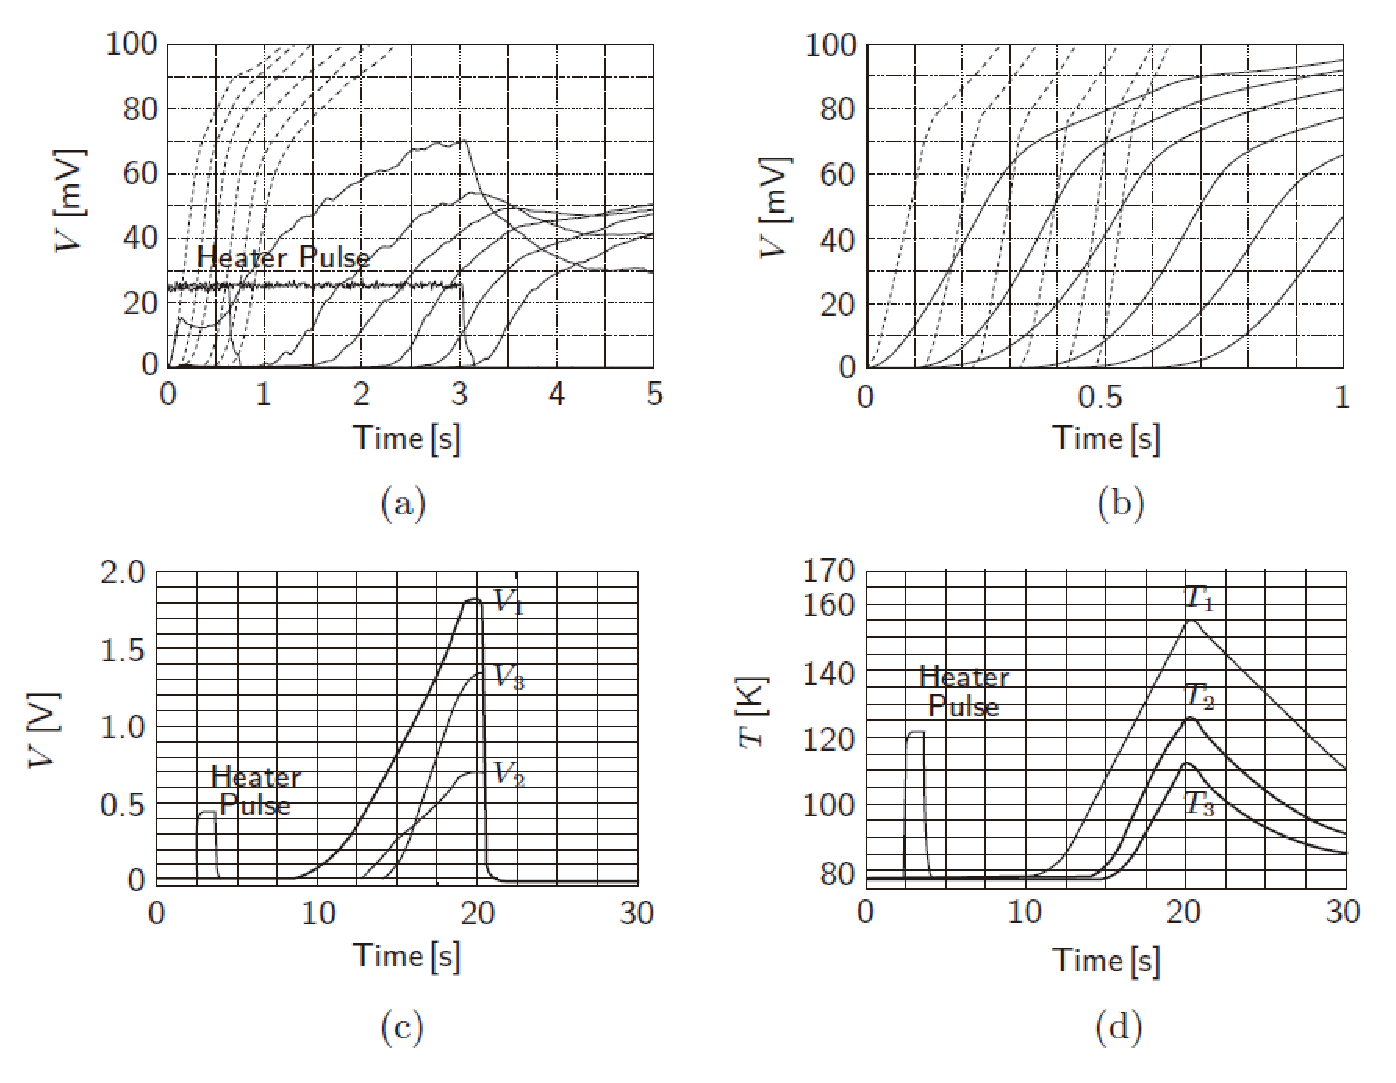
\includegraphics[scale=0.5]{chpt8/figs/fig8.11.eps}
	\caption{YBCO测试样品在77 K时得到的横向NZP信号,失超是由加热脉冲触发的。}
\end{figure}



\subsection{热-流体失超恢复(THQB)}
对于迫流氦冷却的CIC导体,在局部正常区传播速度比迫流氦快时,
会出现热-流体失超恢复(thermal-hydraulic quenchback, THQB)现象。
Luongo等[8.76–8.78; 1.23]最初将之视为CIC导体中失超的其他现象
(内部压力升高、导体末端氦排除等)有关系的一种现象。它通常发生于CIC导体运行在基底电流密度$J_m$
很高,接近导体临界电流的时候。
如讨论6.6将讨论到的,因为在聚变磁体中---CIC导体最重要的大型应用---
CIC导体设计运行在小于$I_m$(方程6.30)良好冷却区间,THQB应该不会成为严重的保护问题。

\subsection{交流损耗诱导的NZP}
到目前为止,我们将焦耳损耗视为绝热绕组中NZP的唯一源。
当非恢复正常区产生并进入故障模式后,磁体电流随时间衰减,衰减电流幅值在$\sim 100$ A/s,进而在绕组中产生时变磁场$dB/dt$---NMR磁体的情况将在问题8.6研究。
时变磁场的存在导致交流损耗的产生;方程6.1中,$g_d(t)\neq 0$。
在没有局部冷却的时候,这个$dB/dt$感应的$g_d(t)$导致在绕组中$\Delta T_{op}>0$。
$g_d(t)$越大,$\Delta T_{op}>0$越大。如6.2.6所述,甚至绝热绕组也能承受一个极限$\Delta T_{op}$,
具体可高至温度裕度极限$[\Delta T_{op}]_{mx}$。
因为这个$g_d(t)$加热,一些NMR磁体以很慢的速率励磁,某些时候会经历一个星期才达到运行电流,
以确保满足绝热稳定性条件$\Delta T_{op}<[\Delta T_{op}]_{mx}$。

因此,$dB/dt$感应的加热令$U_\ell$和$U_t$的视在值明显大于仅有焦耳耗散作为驱动力的NZP。
$dB/dt$感应的加热可以设计用来加速故障事件下的NZP,此时快速扩大正常区并将电流快速降低是很重要的[8.79-8.81]。
为了保护,一些NMR和MRI磁体还使用特殊选定的长绞合节距多丝导体来提高耦合损耗。

在更大的电流衰减率幅值下,比如$\sim 0.1-1$ MA(尽管明显不可能在高感性MRI和NMR磁体中出现,
但在电阻性设备比如限流器中会遇到),Vysotsky等人发现快速NZP接近 1km/s[8.82];
在这种快速电流变化下,失超成为全局的,而不是从局部开始传播的。


\section{计算机仿真}
由于绝热磁体中失超过程的耦合特定,特别是那些多线圈系统,失超分析最好借助计算机来进行。
Wilson在1968年做了早期尝试[8.83],失超仿真工作(一些还引入了实验结果)持续进行[1.5–1.23;8.84–8.100],
一些工作专门针对HTS绕组。

这里我们简要描述FBNML涉及的绝热、螺管绕组的失超仿真程序,该程序的最初工作是1985年Williams[8.101]做的。
FBNML程序简单的认为绕组内控制正常区域传播的复杂热扩散过程可以简化为一个单一参数横向传播速度$U_t$,该参数
依赖于磁场、温度和基底电流密度。
将绕组的热属性的复杂效应归结为$U_t$,极大的简化了程序且没有牺牲很大的准确性[8.45,8.101]。
如8.4.3中讨论的,$U_t$与长度方向的传播速度$U_\ell$有关;
于是,$U_t$在绕组内既与时间有关,也与位置有关。

图8.12给出了绝热螺管绕组内的失超传播示意图,图中的绕组为圆线密排六边形并浸渍了环氧。
图中的失超开始于绕组中平面的最内半径处。
因为下面的对多数磁体都成立的条件,
横向传播速度$U_t$确定的匝间输运时间或通常小于由长度方向传播速度$U_\ell$确定的周向输运时间:
\begin{equation}% 8.56
\frac{d_{cd}}{U_t}\ll\frac{2\pi a_1}{U_\ell}
\end{equation}

\begin{figure}
	\centering
	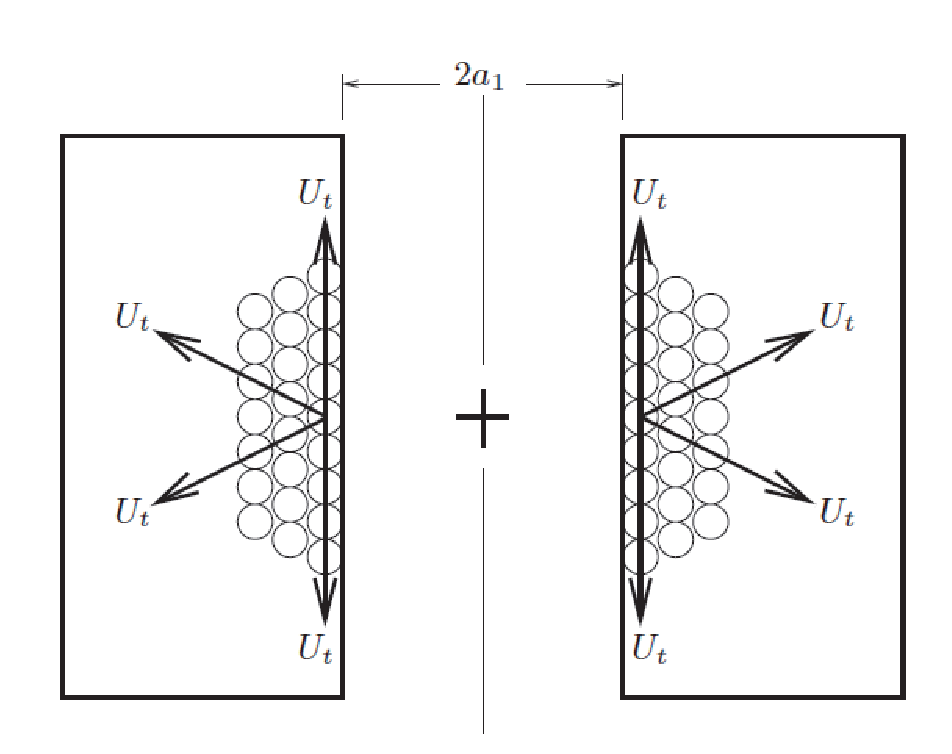
\includegraphics[scale=0.5]{chpt8/figs/fig8.12.eps}
	\caption{绝热螺管绕组中的失超}
\end{figure}

\section{自保护磁体}
如果超导磁体在过热时无需依赖于外部干预即可将正常区域快速扩展到整个绕组,那就称为是自保护的。
根据8.1.2,多数绝热磁体为了保证最高温度低于$\sim 200$ K,至少需要$\sim 10\%$的绕组体积来吸收磁能。
该过程发展的发生快慢可以用NZP速度来衡量。
下面的定性分析将表明,自保护磁体必须有很快的NZP速度且很小。
不过,如后面将讨论的,磁体尽管可以对过热自保护,但不一定能对应力过大保护。

\subsection{尺寸限制}
由8.1.2中的标8.1可见,磁体的初始储能如果完全耗散为绕组中的热量,
为了保持$T_f$在$\sim$200 K以下,绕组的至少$\sim 10\%$($f_r=\sim 0.1$必须
在电流衰减时间$\tau_{dg}$内转变为正常态来吸收能量。

如果在磁体的最内半径$a_1$处产生小正常区,我们需要满足磁体绕组半径$a_1(\alpha-1)$的理想要求来
确保$f_r$足以实现自保护。条件如下:
\begin{equation}% 8.57
\frac{a_1(\alpha-1)}{U_t}<\tau_{dg}
\end{equation}

方程8.57表明整个径向的传播时间$a_1(\alpha-1)/U_t$必须小于$\tau_{dg}$。
实际上,如前所述,不太大的绕组体积分数即足够保持$T_f$在$\sim 200$ K之下。
在这里的“幅值量级”讨论中,我们使用8.57给出的理想条件。

\subsubsection*{恒电流加热下的尺寸限制}
在绝热、恒电流加热模式(8.2.1)下,我们有$\tau_{dg}=\tau_{ah}^i(T_f,T_i)$,其中
$\tau_{ah}^i(T_f,T_i)$由8.12a给出,是绝热恒电流($J_{m_o}$)加热下的最长时间。联立8.57和8.12a,有:
\begin{equation}% 8.58
\frac{a_1(\alpha-1)}{U_t}=\frac{Z(T_f,T_i)}{J_{m_o}^{2}}
\end{equation}

联立8.51b和8.52和8.58,并令$J_m=J_{m_o}$,我们得到绝热恒电流加热条件下的自保护磁体的
绕组尺寸极限$[a_1(\alpha-1)]_{ah}^i$:
\begin{equation}% 8.59
[a_1(\alpha-1)]_{ah}^{i}=\frac{Z(T_f,T_i)}{J_{m_o}C_m(\tilde{T})}\sqrt{\frac{\rho_m(\tilde{T})k_i(\tilde{T})\delta_{cd}}{2\delta_i(T_t-T_{op})}}
\end{equation}

方程8.59表明,允许的磁体尺寸随$J_{m_o}$和$C_m(\tilde{T})$而减小,随$Z(T_f,T_i)$而增大。
它还表明,尺寸极限随$\rho_m(\tilde{T})$和$k_i(\tilde{T})$而增大,随$(T_t-T_{op})$而缩小。
$C_m(\tilde{T})$和$(T_t-T_{op})$的依赖性意味着对同样的$J_{m_o}$和$T_f$,
自保护HTS磁体如果要可以实际应用的话,必须要比LTS更为紧凑才行。

\subsubsection*{端子短接磁体的尺寸限制}
从保护的角度看,让端子短接磁体可以自保护是很有价值的。
实际上,多数NMR和MRI磁体都设计为自保护的。自保护不一定用NZP扩散正常区,而是用
感应交流损耗和二连接于磁体端子的二极管和电阻器。

这里,我们使用仅用NZP的端子短接磁体实现自保护的尺寸极限:
磁体在端子短接下的绝热加热见8.2.3的讨论。
这里,$\tau_{dg}=R_{nz}/L$,其中$R_{nz}$有方程8.27或8.25给出。
联立8.57和8.27,使用8.52和8.51b给出的$U_t$,
解得端子短接自保护磁体在绝热加热时的绕组限制$[a_1(\alpha-1)]_{ah}^{sh}$:
\begin{subequations}% 8.60a 8.60b 8.60c
	\begin{align}
[a_1(\alpha-1)]_{ah}^{sh}=&U_t\left(\frac{L}{R_{nz}}\right) \\
=&\frac{J_{m_o}}{C_n(\tilde{T})}\sqrt{\frac{\rho_m(\tilde{T})k_i(\tilde{T})\delta_{cd}}{2\delta_i(T_t-T_{op})}}\left(\frac{L}{R_{nz}}\right)  \\
=&\frac{J_{m_o}}{C_n(\tilde{T})}\sqrt{\frac{\rho_m(\tilde{T})k_i(\tilde{T})\delta_{cd}}{2\delta_i(T_t-T_{op})}}\times \\\notag
&\frac{4A_m}{f_r\pi(\alpha+1)\rho_m(T_f)}\sqrt{\frac{\mu_o\mathcal{L}(\alpha,\beta)L}{a_1}}\\
[a_1(\alpha-1)]_{ah}^{sh}=&\frac{1}{C_m(\tilde{T})}\sqrt{\frac{\rho_m(\tilde{T})k_i(\tilde{T})\delta_{cd}}{2\delta_i(T_t-T_{op})}}\times \\\notag
&\frac{4}{f_r\pi(\alpha+1)\rho_m(T_f)}\sqrt{\frac{2\mu_o\mathcal{L}(\alpha,\beta)E_m}{a_1}}
\end{align}
\end{subequations}

类似的,在如上面处理的恒电流加热模式下,因为$C_m(\tilde{T})$和$(T_t-T_{op})$出现在8.60c和8.60d的分母中,
在同样的运行参数下,自保护HTS磁体必须要比运行于液氦温度的LTS尺寸更小。


\section{孤立磁体的被动保护}

\begin{equation}% 8.61
\frac{E_r}{E_m}=\frac{0.5\zeta(1-k)+(1+k)}{\zeta+(1+k)}
\end{equation}


\begin{figure}
	\centering
	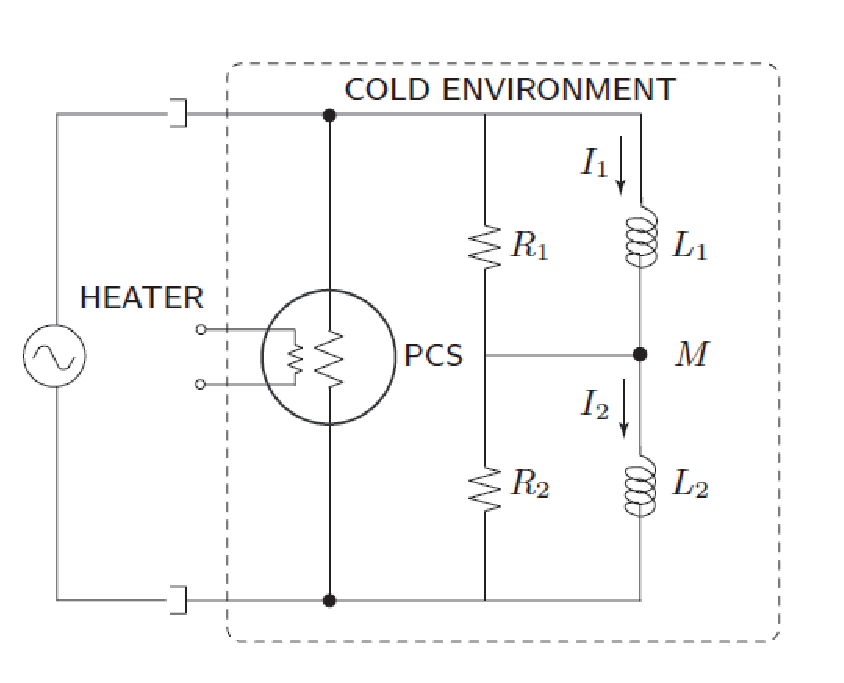
\includegraphics[scale=0.6]{chpt8/figs/fig8.13.eps}
	\caption{Circuit for an “isolated,” persistent-mode 2-coil magnet.}
\end{figure}





\begin{equation}% 8.62a
\frac{I_1(t)}{I_0}=\frac{R(1+k)^2}{2r}\exp\left(-\frac{Rt}{2L}\right)\left[1-\frac{R(1+k)^2}{2r}\right]\exp\left[-\frac{rt}{(1-k^2)L}\right]
\end{equation}
\begin{equation}% 8.62b
\frac{I_2(t)}{I_0}=(1+k)\exp\left(-\frac{Rt}{2L}\right)-k\exp\left[-\frac{rt}{(1-k^2)L}\right]
\end{equation}


\begin{figure}
	\centering
	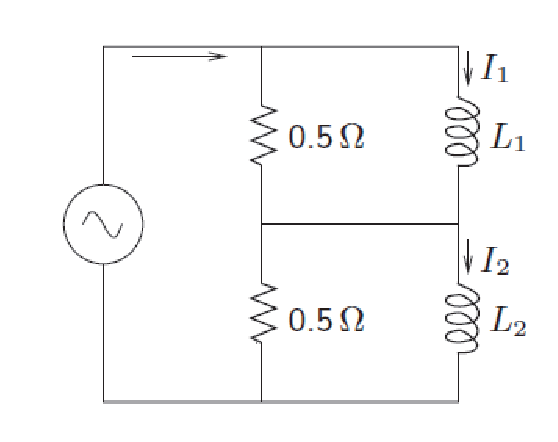
\includegraphics[scale=0.6]{chpt8/figs/fig8.14.eps}
	\caption{2-Coil Magnet circuit}
\end{figure}





\begin{figure}
	\centering
	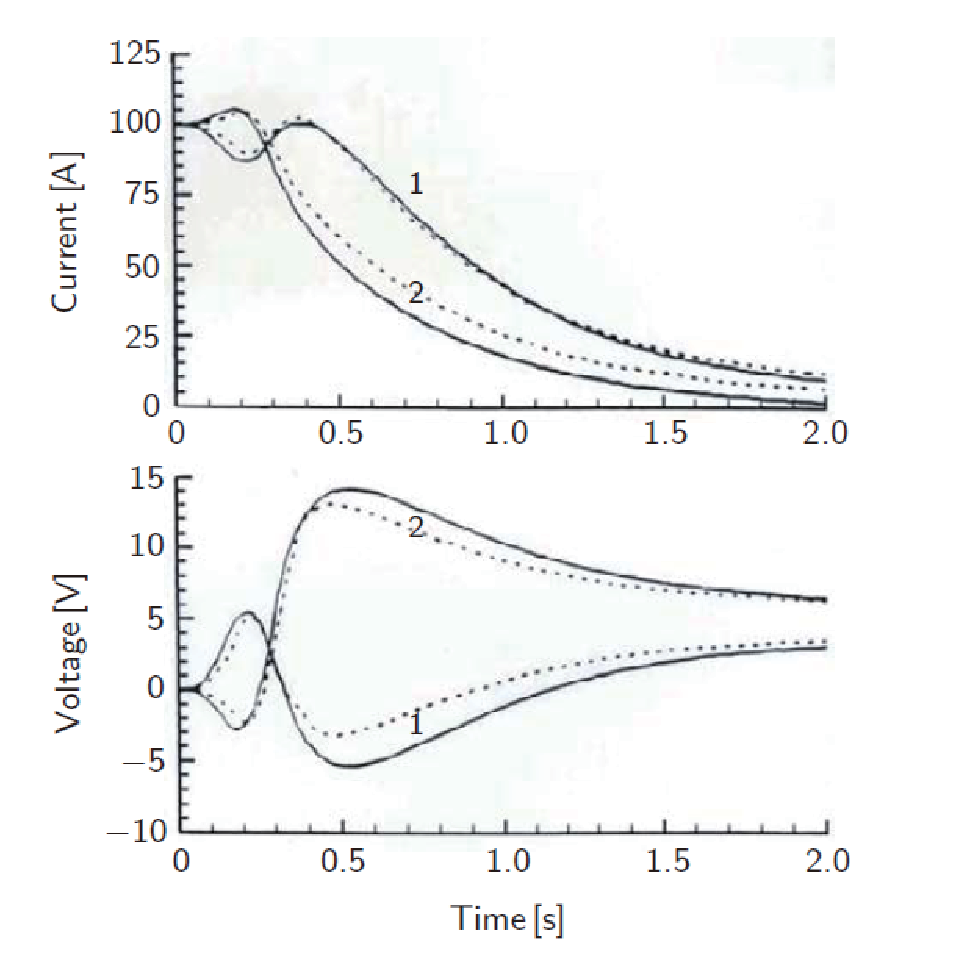
\includegraphics[scale=0.6]{chpt8/figs/fig8.15.eps}
	\caption{Current and voltage vs. time traces of Coil 1 }
\end{figure}







\begin{equation}% 8.63
E_d=E_m+E_s-E_{R1}-E_{R2}
\end{equation}

\begin{align*}% page500第一个
E_s&=(100\ \mathrm{A})\int_{0}^{0.4\ \mathrm{s}}[V_1(t)+V_2(t)]dt+(10\ \mathrm{V})\int_{0.4\ \mathrm{s}}^{2\ \mathrm{s}}\left[I_1(t)+\frac{V_1(t)}{R_1}\right]dt \\
&\simeq 200\ \mathrm{J}+650\ \mathrm{J}\simeq 850\ \mathrm{J}
\end{align*}


\begin{equation}% page500 第二个和第三个
E_{R1}=\frac{1}{R_1}\int_{0}^{2\ \mathrm{s}}V_1(t)^2dt\simeq 50\ \mathrm{J} 
E_{R2}=\frac{1}{R_2}\int_{0}^{2\ \mathrm{s}}V_2(t)^2dt\simeq 300\ \mathrm{J}
\end{equation}

\begin{equation}% page500第四个
\mathcal{V}_{cd}[h_{cu}(T_f)-h_{cu}(T_{op})]\simeq(694\ \mathrm{cm^3})[h_{cu}(T_f)]=5500\ \mathrm{J}
\end{equation}




\begin{figure}
	\centering
	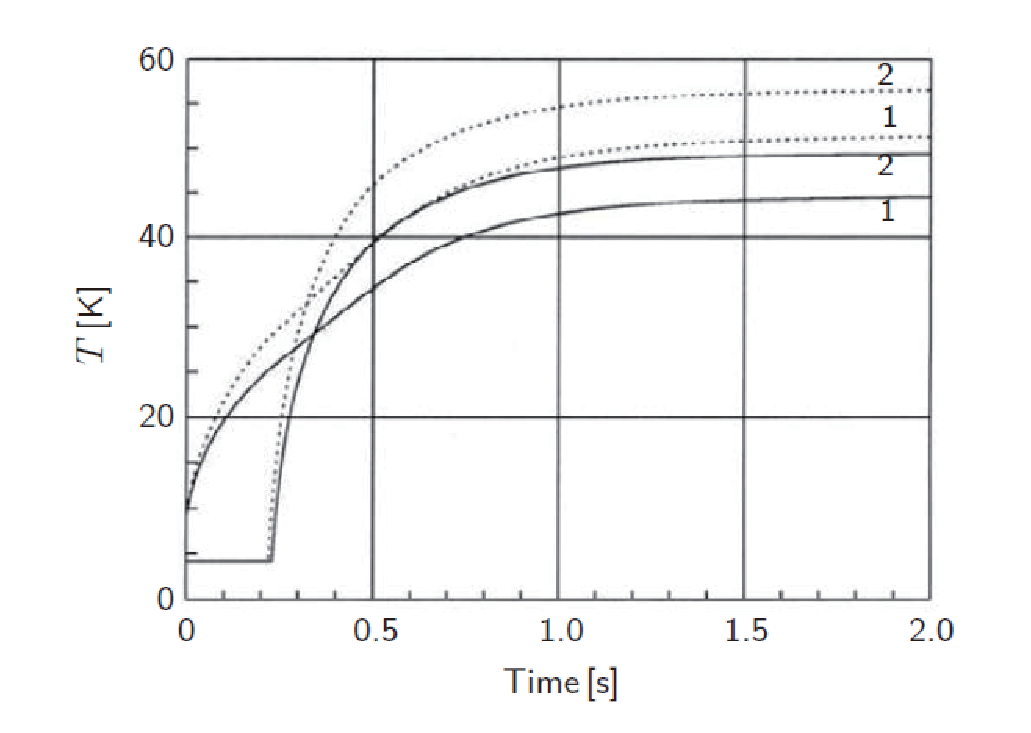
\includegraphics[scale=0.6]{chpt8/figs/fig8.16.eps}
	\caption{Spatially averaged temperature vs. time plots for Coils 1 and 2 }
\end{figure}







\section{主动保护}
\subsection{过热}
\begin{equation}% page501 8.7
e_{mr}\equiv\frac{E_m}{V_r}=\frac{2(\alpha-1)\beta\mathcal{L}(\alpha,\beta)}{f_r\pi(\alpha+1)F^2(\alpha,\beta)}\left(\frac{B_{o}^{2}}{2\mu_o}\right)
\end{equation}


\subsection{多线圈磁体中的过压}


\subsection{主动保护技术:检测-抑制}

\begin{equation}% page502 8.18b
Z(T_f,T_i)=\frac{J_{m_o}E_m}{A_{cd}V_D}
\end{equation}

\begin{figure}
	\centering
	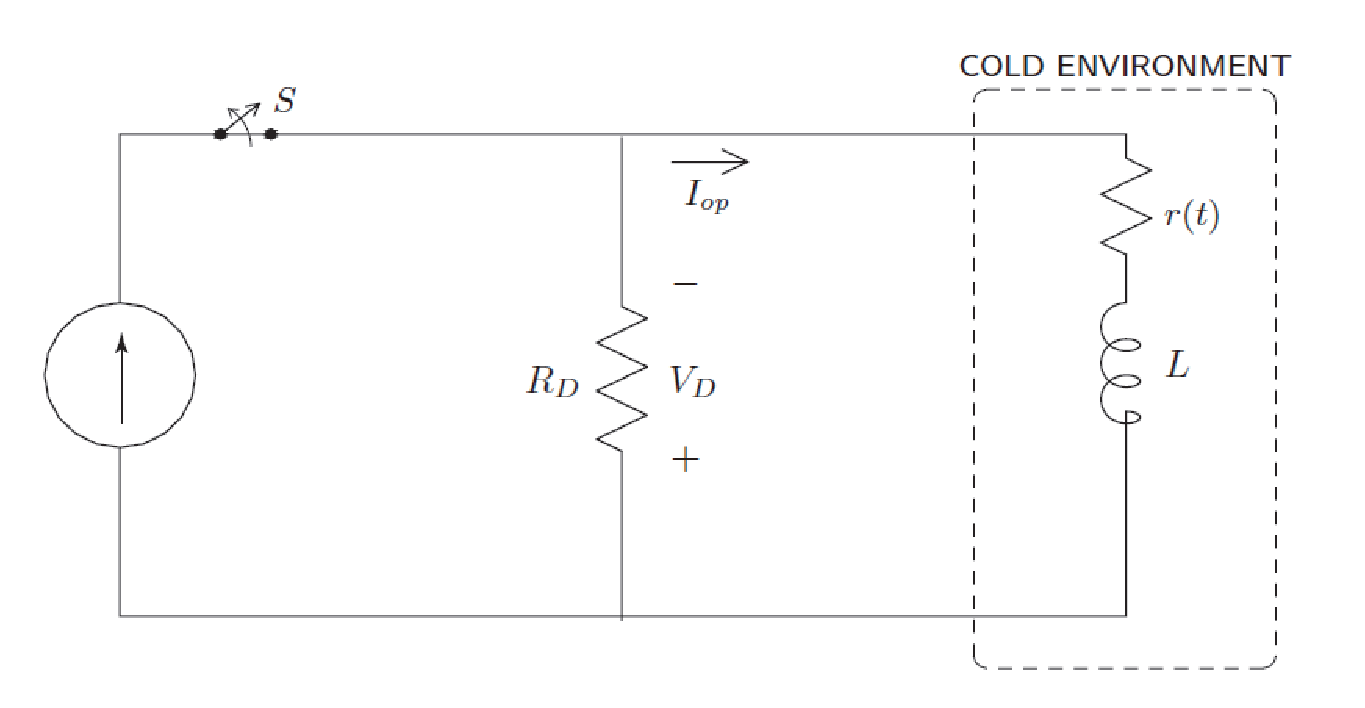
\includegraphics[scale=0.6]{chpt8/figs/fig8.17.eps}
	\caption{Magnet circuit for detect-and-dump active protection}
\end{figure}



\begin{equation}% page503 8.19
J_{m_o}^{D}=\frac{A_{cd}Z(T_f,T_i)V_D}{E_m}
\end{equation}



\begin{equation}% 8.65
V_D=\frac{J_{m_o}E_m}{A_{cd}Z(T_f,T_i)}
\end{equation}
\begin{equation}% 8.66a 8.66b
Z(T_f,T_i)=\left(\frac{A_m}{A_{cd}}\right)(J_{m_o}^{2}\tau_{dl}+\frac{1}{2}J_{m_o}^{2}\tau_{dg})
=\left(\frac{A_m}{A_{cd}}\right)(\tau_{dl}+\frac{1}{2}\tau_{dg})J_{m_o}^{2}
\end{equation}






\subsection{主动保护技术:检测-激活加热器}

\begin{figure}
	\centering
	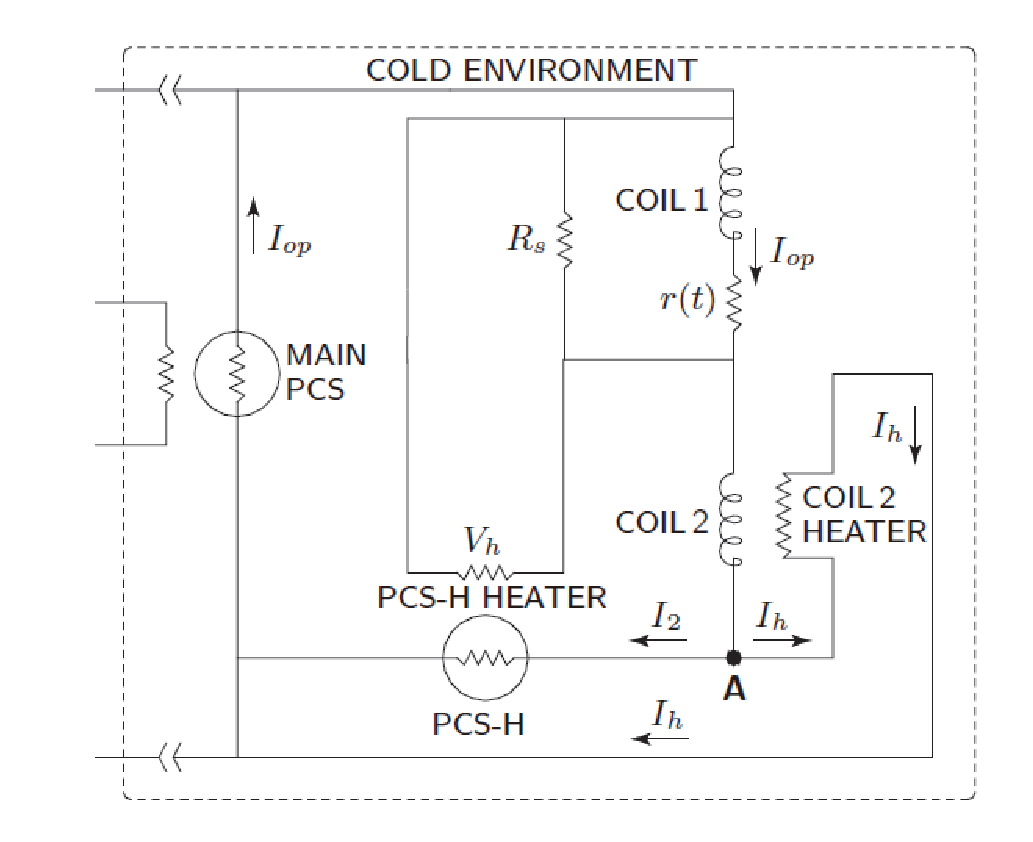
\includegraphics[scale=0.6]{chpt8/figs/fig8.18.eps}
	\caption{Magnet circuit with passive activate-the-heater protection.}
\end{figure}




\subsection{失超电压保护技术:基本电桥}


\begin{figure}
	\centering
	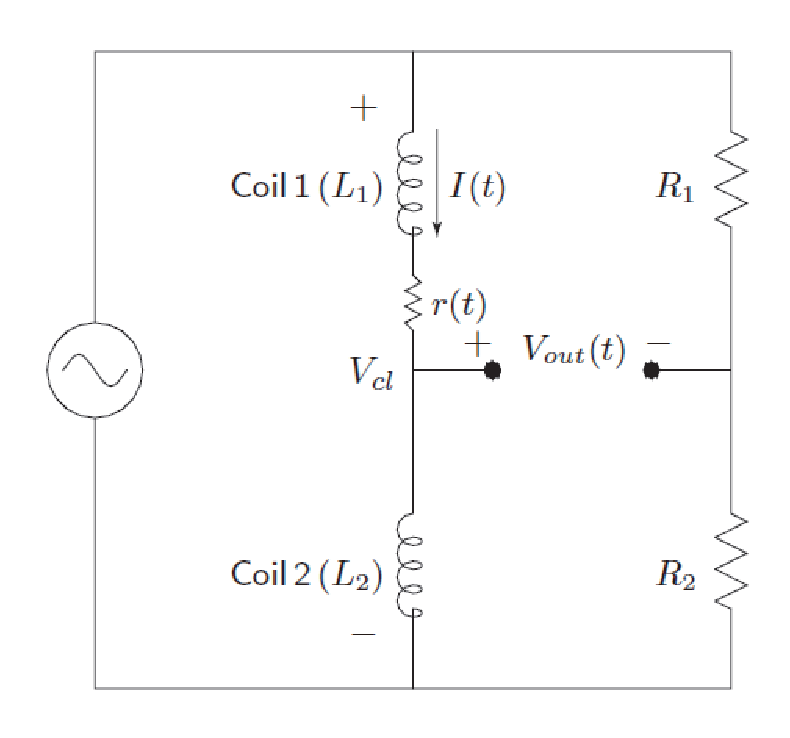
\includegraphics[scale=0.6]{chpt8/figs/fig8.19.eps}
	\caption{Bridge circuit voltage detection technique}
\end{figure}


\begin{equation}% 8.67a
V_{cl}(t)=L_1\frac{dI(t)}{dt}+rI(t)+L_2\frac{dI(t)}{dt}
\end{equation}
\begin{equation}% 8.67b
i_R(t)=\frac{V_{cl}(t)}{R_1+R_2}
\end{equation}
\begin{equation}% 8.67c
V_{out}(t)=L_1\frac{dI(t)}{dt}+rI(t)-R_1i_R(t)
\end{equation}


\begin{align}% 8.68
V_{out}(t)&=L_1\frac{dI(t)}{dt}+rI(t) 
-\frac{R_1}{R_1+R_2}\left[L_1\frac{dI(t)}{dt}+rI(t)+L_2\frac{dI(t)}{dt}\right] \\\notag
&=\left(\frac{R_2}{R_1+R_2}\right)L_1\frac{dI(t)}{dt} 
-\left(\frac{R_1}{R_1+R_2}\right)L_2\frac{dI(t)}{dt}+\left(\frac{R_2}{R_1+R_2}\right)rI(t)
\end{align}



\begin{equation}% 8.69
\left(\frac{R_2}{R_1+R_2}\right)L_1\frac{dI(t)}{dt}-\left(\frac{R_1}{R_1+R_2}\right)L_2\frac{dI(t)}{dt}=0
\end{equation}


\begin{equation}% 8.70
V_{out}(t)=\left(\frac{R_2}{R_1+R_2}\right)rI(t)
\end{equation}


\section{专题}

\subsection{问题8.1:大型超导磁体的回温}
\begin{equation}% 8.71a 8.71b
\mathcal{V}C_{cd}(T)\frac{dT}{dt}=\frac{\rho_m(T)\ell_{cd}}{A_m}I_{o}^{2} 
=\frac{A_m}{\rho_m(T)\ell_{cd}}V_{o}^{2}
\end{equation}

\subsubsection{问题8.1之解}
\begin{align*}% page508 S1.1
\Delta t_{\omega}^{I}\mid_{10\ \mathrm{K}}^{300\ \mathrm{K}}&=\frac{\mathcal{V}_{cd}A_m}{\ell_{cd}I_{o}^{2}}\int_{10\ \mathrm{K}}^{300\ \mathrm{K}}\frac{C_{cu}(T)}{\rho_m{cu}(T)}dT \\
&=\frac{\mathcal{V}_{cd}A_m}{\ell_{cd}I_{o}^{2}}Z(T_f=300\ \mathrm{K},T_i=10\ \mathrm{K})
\end{align*}


\begin{align*}% page508 S1.2
\Delta t_{\omega}^{I}\mid_{10\mathrm{K}}^{300\mathrm{K}}&=\frac{(0.4\ \mathrm{m^3})(1.5\times 10^{-5}\ \mathrm{m^2})(15.1\times 10^{16}\ \mathrm{A^2s/m^4})}{(1\times 10^4\ \mathrm{m})(25\ \mathrm{A})^2} \\
&\simeq 1.45\times 10^5\ \mathrm{s}\simeq 40\ \mathrm{h}\simeq 1\frac{2}{3}\ \mathrm{days} 
\end{align*}


\begin{align*}% page508 S1.3
\Delta t_{\omega}^{I}\mid_{10\mathrm{K}}^{300\mathrm{K}}&=\frac{\mathcal{V}_{cd}\ell_{cd}}{A_mV_{o}^{2}}\int_{10\ \mathrm{K}}^{300\ \mathrm{K}}C_{cu}(T)\rho_m{cu}(T)dT \\
&=\frac{\mathcal{V}_{cd}\ell_{cd}}{A_mV_{o}^{2}}Y(T_f=300\ \mathrm{K},T_i=10\ \mathrm{K})
\end{align*}


\begin{align*}% page508 S1.4
\Delta t_{\omega}^{I}\mid_{10\mathrm{K}}^{300\mathrm{K}}&=\frac{(0.4\ \mathrm{m^3})(1\times 10^4\ \mathrm{m})(7.25\ \mathrm{V^2s/m^2})}{(1.5\times 10^{-5}\ \mathrm{m^2})(25\ \mathrm{V})^2} \\
&=3.1\times 10^6\ \mathrm{s}\simeq 860\ \mathrm{h}\simeq 36\ \mathrm{days} 
\end{align*}


\begin{align*}% page509 S1.5
\Delta t_{\omega}^{I}\mid_{10\mathrm{K}}^{50\mathrm{K}}&=\frac{(0.4\ \mathrm{m^3})(1.5\times 10^{-5}\ \mathrm{m^2})(4.5\times 10^{16}\ \mathrm{A^2s/m^4})}{(1\times 10^4\ \mathrm{m})(100\ \mathrm{A})^2} \\
&\simeq 2.7\times 10^3\ \mathrm{s}=45\ \mathrm{min}
\end{align*}


\begin{equation}% page509 S1.6
\Delta t_{\omega}^{I}\mid_{50\mathrm{K}}^{300\mathrm{K}}=\frac{(0.4\ \mathrm{m^3})(1\times 10^4\ \mathrm{m})(7.25\ \mathrm{J\Omega/m^2})}{(1.5\times 10^{-5}\ \mathrm{m^2})(100\ \mathrm{V})^2} 
=1.93\times 10^5\ \mathrm{s}=54\ \mathring{h}
\end{equation}
\begin{equation}% page509 S1.7
\Delta t_{\omega}^{I}\mid_{80\mathrm{K}}^{300\mathrm{K}}\simeq 0.7\times 10^5\ \mathrm{s}\sim 20\ \mathrm{h}
\end{equation}
\begin{equation}% page509 S1.8
\Delta t_{\omega}^{I}\mid_{80\mathrm{K}}^{300\mathrm{K}}\simeq 3\times 10^6\ \mathrm{s}\simeq 830\ \mathrm{h}\simeq 35\ \mathrm{days}
\end{equation}



\subsection{问题8.2:6 kA气冷HTS引线的保护}


\subsubsection{问题8.2之解}
\begin{equation}% 8.66b
Z(T_f,T_i)=\left(\frac{A_m}{A_{cd}}\right)(\tau_{dl}+\frac{1}{2}\tau_{dg})J_{o}^{2}
\end{equation}
\begin{equation}% page510 S.1
Z(T_f,T_i)=\left(\frac{\gamma_{m/s}}{1+\gamma_{m/s}}\right)(\tau_{dl}+\frac{1}{2}\tau_{dg})J_{o}^{2}
\end{equation}
\begin{equation}% page510 第三个
Z(T_f,T_i)=(12.5\ \mathrm{s})\left(\frac{2}{3}\right)(3.46\times 10^7\ \mathrm{A/m^2})^2\simeq 1\times 10^{16}\ \mathrm{A^2s/m^4}
\end{equation}



\subsection{问题8.3:制冷机制冷的NbTi磁体的保护}

\subsubsection{问题8.3之解}
\begin{equation}% page511 第一个
I_{op}=(6.25\times 10^7\ \mathrm{A/m^2})\frac{(10\times 10^{-3}\ \mathrm{m})(3\times 10^{-3}\ \mathrm{m})4}{(1+4)}=1500\ \mathrm{A}
\end{equation}
\begin{equation}% 8.72
V_D=\frac{J_{m_o}E_m}{A_{cd}Z(T_f,T_i)}
\end{equation}
\begin{equation}% page511 S3.1
V_D=\frac{(6.25\times 10^7\ \mathrm{A/m^2})^2(10\times 10^6\ \mathrm{J})}{(3\times 10^{-5}\ \mathrm{m^2})(6.7\times 10^{16}\ \mathrm{A^2s/m^4})} 
=310\ \mathrm{V}
\end{equation}



\subsection{问题8.4:混合III SCM的“热点”温度}
\begin{equation}% 8.73
r(t)=r_0+\eta t
\end{equation}
\begin{equation}% 8.74
I(t)=I_{op}\exp\left[-\frac{(R_D+r_0)}{L}t-\frac{\eta}{2L}t^2\right]
\end{equation}


\subsubsection{问题8.4之解}

\begin{equation}% page513 8.16c
Z(T_f,T_i)=\left(\frac{\gamma_{m/s}}{1+\gamma_{m/s}}\right)J_{m_o}^{2}\left(\frac{L}{2R_D}\right)
\end{equation}
\begin{equation}% page513 S4.1
J_{m_o}=\frac{I_{op}}{A_m}=\left(\frac{\gamma_{m/s}+1}{\gamma_{m/s}}\right)\frac{I_{op}}{ab}
\end{equation}
\begin{equation}% page513 S4.2
J_{m_o}=\left(\frac{5.1}{4.1}\right)\frac{(2230\ \mathrm{A})}{(9.49\times 10^{-3}\ \mathrm{m})(4.52\times 10^{-3}\ \mathrm{m})} 
=6.47\times 10^7\ \mathrm{A/m^2}
\end{equation}
\begin{equation}% page513 S4.2后第一个
Z(T_f,4\ \mathrm{K})=\left(\frac{5.1}{4.1}\right)(6.47\times 10^7\ \mathrm{A/m^2})^2\left(\frac{8\ \mathrm{H}}{2\times 0.3\Omega}\right)
\end{equation}
\begin{equation}% page513 S4.2后第二个
Z(T_f,4\ \mathrm{K})=4.5\times 10^{16}\ \mathrm{A^2s/m^4}
\end{equation}
\begin{equation}% page513 S4.3
L\frac{dI(t)}{dt}+(R_D+R_0+\eta t)I(t)=0
\end{equation}
\begin{equation}% page513 S4.4
\frac{dI(t)}{dt}=-\frac{(R_D+R_0+\eta t)}{L}dt
\end{equation}
\begin{equation}% page513 S4.5
\ln\left[\frac{I(t)}{I_{op}}\right]=-\frac{(R_D+R_0)}{L}t-\frac{\eta}{2L}t^2
\end{equation}
\begin{equation}% 8.74
I(t)=I_{op}\exp\left[-\frac{(R_D+R_0)}{L}t-\frac{\eta}{2L}t^2\right]
\end{equation}
\begin{equation}% page514 S4.6
E_{sm}\int_{0}^{\infty}r(t)I_{0}^{2}\exp\left[-\frac{2(R_D+R_0)}{L}t-\frac{\eta}{L}t^2\right]dt
\end{equation}

\subsection{讨论8.1:失超电压探测——一个变种}


\begin{figure}
	\centering
	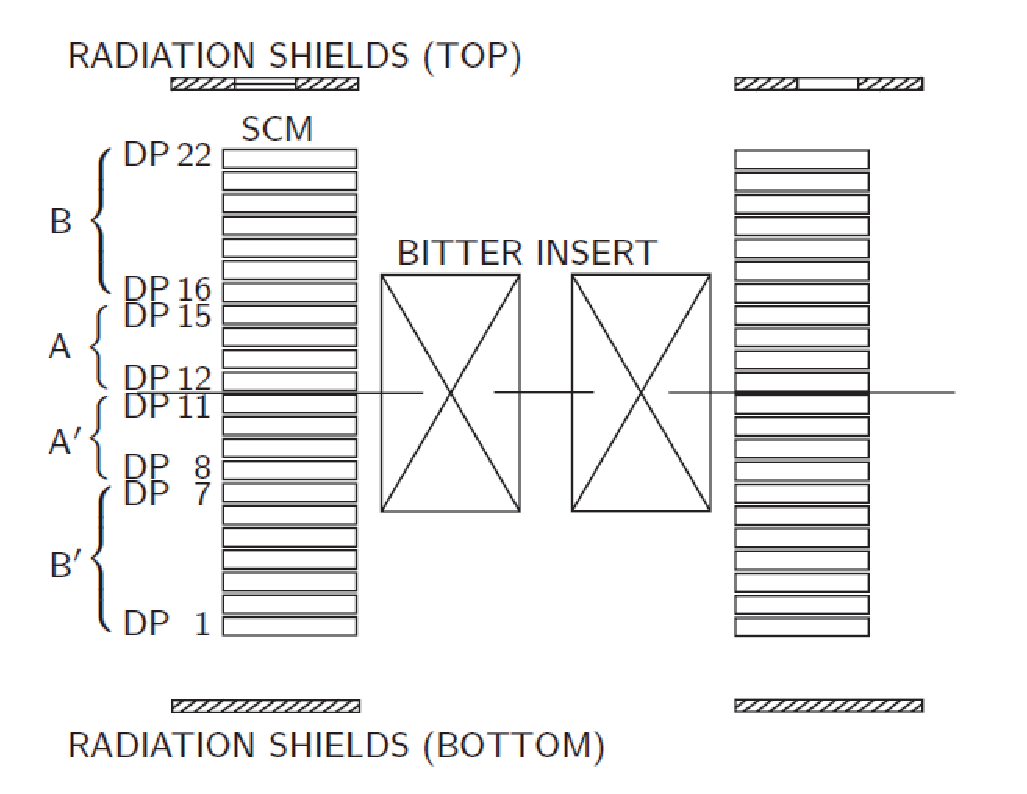
\includegraphics[scale=0.6]{chpt8/figs/fig8.20.eps}
	\caption{Schematic arrangement of Hybrid II with a Bitter insert}
\end{figure}




\begin{equation}% 8.75
V_{out}(t)=\sum_{n=1}^{11}[\alpha_{2n-1}V_{2n-1}(t)-\alpha_{2n}V_{2n}(t)]
\end{equation}

\begin{figure}
	\centering
	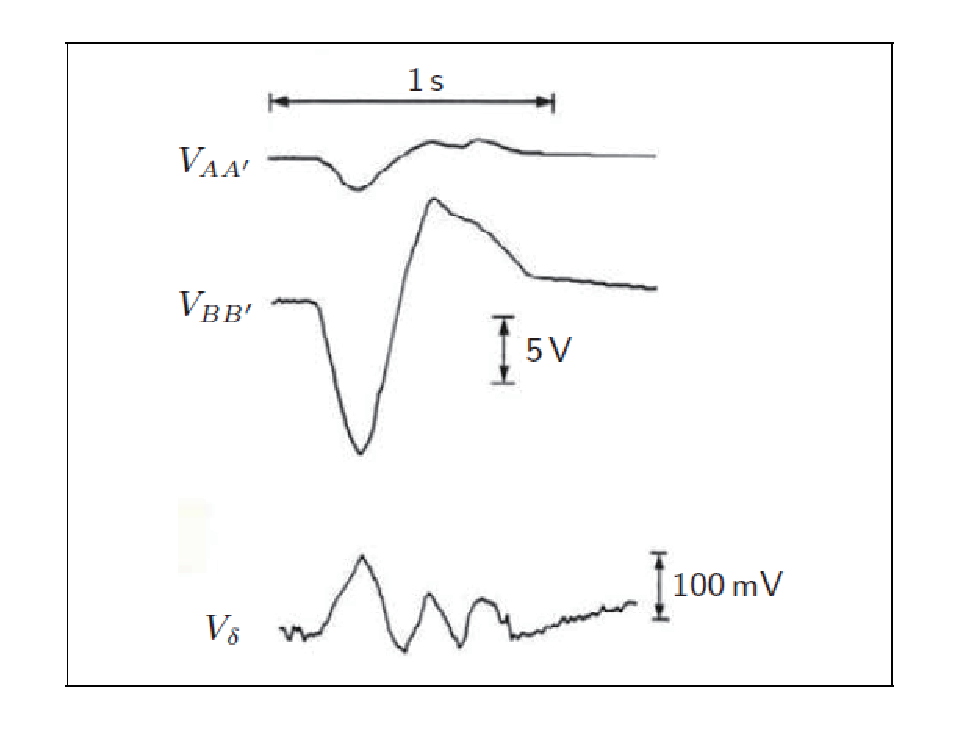
\includegraphics[scale=0.6]{chpt8/figs/fig8.21.eps}
	\caption{Measured unbalanced voltages from an insert trip in Hybrid II}
\end{figure}



\subsection{问题8.5:抑制电阻的设计}
\begin{equation}% 8.76a
\ell=\sqrt{\frac{E_mR_D}{\rho C_p\Delta T}}
\end{equation}
\begin{equation}% 8.76b
\omega\delta=\sqrt{\frac{\rho E_m}{R_DC_p\Delta T}}
\end{equation}

\begin{figure}
	\centering
	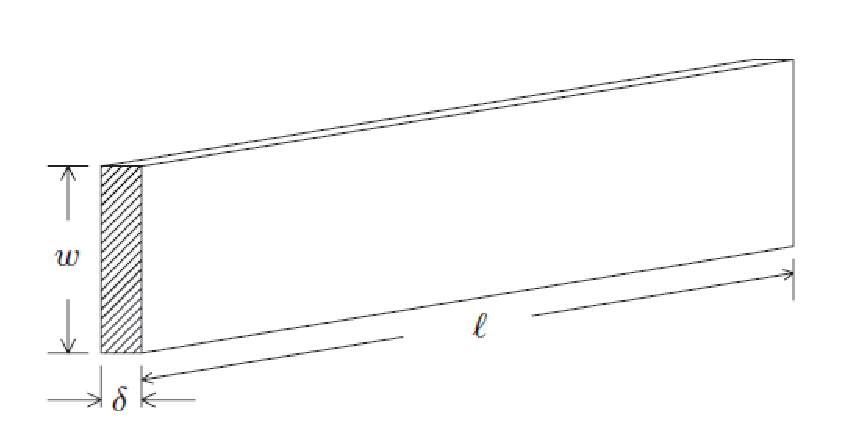
\includegraphics[scale=0.6]{chpt8/figs/fig8.22.eps}
	\caption{Schematic drawing of a dump resistor in the form of a}
\end{figure}






\subsubsection{问题8.5之解}

\begin{equation}% page518 S5.1a
R_D-\frac{\rho\ell}{\omega\delta}
\end{equation}
\begin{equation}% page518 S5.1b
\omega\delta=\frac{\rho\ell}{R_D}
\end{equation}
\begin{equation}% page518 S5.2a
E_m=\ell\omega\delta C_p\Delta T
\end{equation}
\begin{equation}% page518 S5.2b
\omega\delta=\frac{E_m}{\ell C_p\Delta T}
\end{equation}
\begin{equation}% 8.76a
\omega\delta=\sqrt{\frac{\rho E_m}{R_DC_p\Delta T}}
\end{equation}
\begin{equation}% page518 倒数第二个
\ell\simeq\sqrt{\frac{(2\times 10^7\ \mathrm{J})(0.3\Omega)}{(10^{-6}\ \mathrm{\Omega m})(4\times 1066\ \mathrm{J/m^2K})(200\ \mathrm{K})}} 
=86.6\ \mathrm{m}
\end{equation}
\begin{align*}% page518 最后一个
\omega\delta&\simeq\sqrt{\frac{(10^{-6}\ \mathrm{\Omega m})(2\times 10^7\ \mathrm{J})}{(0.3\Omega)(4\times 10^6\ \mathrm{J/m^2K})(200\ \mathrm{K})}} \\
&\simeq 2.9\times 10^{-4}\ \mathrm{m^2}\simeq 290\ \mathrm{mm^2}
\end{align*}


\subsection{讨论8.2:磁体的“缓慢”放电模式}
\begin{equation}% 8.77a
\frac{dI_m(t)}{dt}=-\frac{I_m(t)}{\tau_m}
\end{equation}


\begin{figure}
	\centering
	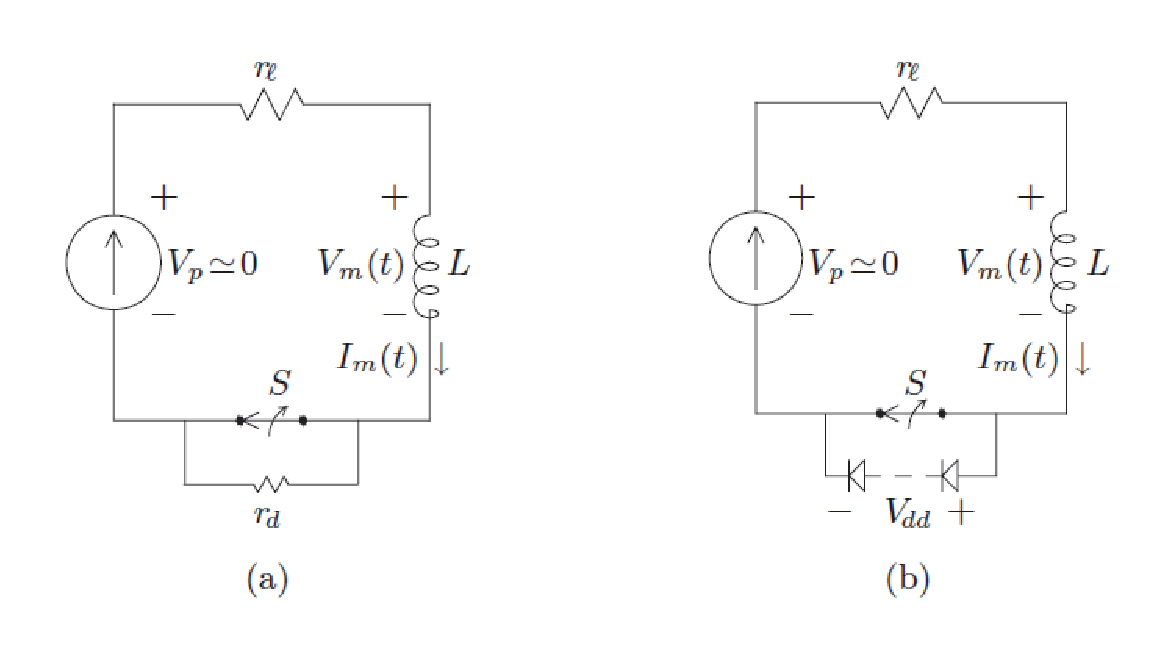
\includegraphics[scale=0.6]{chpt8/figs/fig8.23.eps}
	\caption{Circuits for “slow” discharge modes: (a}
\end{figure}






\begin{equation}% 8.77b
\frac{dI_m(t)}{dt}=-\frac{V_{dd}}{L}
\end{equation}


\subsection{讨论8.3:低阻电阻器设计}
\begin{equation}% 8.78a
r_d=\frac{\rho\ell}{\omega\delta}
\end{equation}
\begin{equation}% 8.78b
r_dI_m(0)^2\simeq 2\omega\ell g_{cv}
\end{equation}
\begin{equation}% 8.79a
\ell\simeq r_dI_m(0)\sqrt{\frac{\delta}{2\rho g_{cv}}}
\end{equation}
\begin{equation}% 8.79b
\omega\simeq I_m(0)\sqrt{\frac{\rho}{2\delta g_{cv}}}
\end{equation}
\begin{equation}% page521 第一个
\ell\simeq(0.01\Omega)(250\ \mathrm{A})\sqrt{\frac{(250\times 10^{-6}\ \mathrm{m})}{2(10^{-6}\ \mathrm{\Omega m})(20\ \mathrm{W/m^2})}} 
\simeq 6.3\ \mathrm{m}
\end{equation}
\begin{equation}% page521 第二个
\omega\simeq(250\ \mathrm{A})\sqrt{\frac{(10^{-6}\ \mathrm{\Omega m})}{2(250\times 10^{-6}\ \mathrm{m})(20\ \mathrm{W/m^2})}} 
\simeq 2.5\ \mathrm{m}
\end{equation}
\begin{equation}% page521第三个
\ell\simeq(0.01\Omega)(250\ \mathrm{A})\sqrt{\frac{(250\times 10^{-6}\ \mathrm{m})}{2(10^{-6}\ \mathrm{\Omega m})(20\times 10^3\ \mathrm{W/m^2})}} 
\simeq 20\ \mathrm{cm}
\end{equation}
\begin{equation}% page521 第四个
\omega\simeq(250\ \mathrm{A})\sqrt{\frac{(10^{-6}\ \mathrm{\Omega m})}{2(250\times 10^{-6}\ \mathrm{m})(20\times 10^3\ \mathrm{W/m^2})}} 
\simeq 8\ \mathrm{cm}
\end{equation}


\subsection{讨论8.4:过热\& 内部电压判据}

\begin{align*}% page522 8.30a
J_{m_{op}}^{sh}&=\left(\frac{1+\gamma_{m/s}}{\gamma_{m/s}}\right)\frac{f_r\pi(\alpha+1)\rho_m(T_f)Z(T_f,T_i)}{2}\sqrt{\frac{a_1}{2\mu_o\ \mathcal{L}(\alpha,\beta)E_m}} \\
&=\left(\frac{1+1}{1}\right)\frac{(0.5)\pi(1.3+1)(1.11\times 10^{-8}\ \mathrm{\Omega m})(10.5\times 10^{16}\ \mathrm{A^2s/m^4})}{2}\times \\
&=\sqrt{\frac{0.15\ \mathrm{m}}{2(4\pi\times 10^{-7}\ \mathrm{H/m})(0.54)(3\times 10^6\ \mathrm{J})}} \\
&\simeq 2(21.1\times 10^8\ \mathrm{J/m^3})(0.19\ \mathrm{Am/J})\\
&\simeq 805\ \mathrm{MA/m^2}=805\ \mathrm{A/mm^2}
\end{align*}



\begin{align*}% 8.40b
J_{m_{op}}^{V}&=\frac{2}{f_r(1-f_r)}\left[\frac{\sqrt{\mathcal{L}(\alpha,\beta)}}{\pi(\alpha+1)}\right]\left[\frac{V_{bk}I_{op}}{\rho_m(T_f)}\sqrt{\frac{2\mu_o}{a_1E_m}}\right] \\
&=\frac{2}{0.5(1-0.5)}\left[\frac{\sqrt{0.54}}{\pi(1.3+1)}\right]\left[\frac{(10^4\ \mathrm{V})(300\ \mathrm{A})}{(1.11\times 10^{-8}\ \mathrm{\Omega m})}\sqrt{\frac{2(4\pi\times 10^{-7}\ \mathrm{H/m})}{(0.15\ \mathrm{m})(3\times 10^6\ \mathrm{J})}}\right] \\
&=8(0.102)(2.70\times 10^{14}\ \mathrm{A^2/m})(2.36\times 10^{-6}\ \mathrm{A^{-1}m^{-1}}) \\
&=5.2\times 10^8\ \mathrm{A/m^2}=520\ \mathrm{A/mm^2}
\end{align*}


\subsection{讨论8.5:Bi2223带电流引线的保护}

\begin{equation}% 8.80
a_mk_m\frac{d^2T}{dz^2}+\frac{\rho_mI_{t}^{2}}{a_m}=0
\end{equation}
\begin{equation}% 8.81
T(\zeta)=T_{cl}+(T_{wm}-T_{cl})\zeta+\frac{\rho_m\ell^2I_{t}^{2}}{2a_{m}^{2}k_m}(\zeta-\zeta^2)
\end{equation}
\begin{equation}% 8.82a
\zeta(T_{pk})=\frac{1}{2}+\frac{a_{m}^{2}k_m}{\rho_mI_{t}^{2}\ell^2}(T_{wm}-T_{cl})
\end{equation}
\begin{equation}% 8.82b
T_{pk}\simeq \frac{1}{2}(T_{cl}+T_{wm})+\frac{\rho_mI_{t}^{2}\ell^2}{8a_{m}^{2}k_m}
\end{equation}
\begin{equation}% page523 最后一个
\frac{a_{m}^{2}k_m}{\rho_mI_{t}^{2}\ell^2}(T_{wm}-T_{cl})=\frac{(8\times 10^{-3}\ \mathrm{cm^2})^2(2\ \mathrm{W/cm K})}{(1\times 10^{-6}\ \mathrm{\Omega cm})(50\ \mathrm{A})^2(15\ \mathrm{cm})^2} 
\simeq 0.01
\end{equation}
\begin{equation}% page524 第一个
T_{pk}\simeq\frac{1}{2}(T_{cl}+\frac{\rho_mI_{t}^{2}\ell^2}{8a_{m}^{2}k_m} 
=\frac{1}{2}(10\ \mathrm{K}+70\ \mathrm{K})+\frac{(1\times 10^{-6}\ \mathrm{\Omega cm})(50\ \mathrm{A})^2(15\ \mathrm{cn})^2}{8(8\times 10^{-3}\ \mathrm{cm^2})^2(2\ \mathrm{W/cm K})}\simeq 590\ \mathrm{K}
\end{equation}



\subsection{讨论8.6:$MgB_2$磁体的主动保护}



\begin{figure}
	\centering
	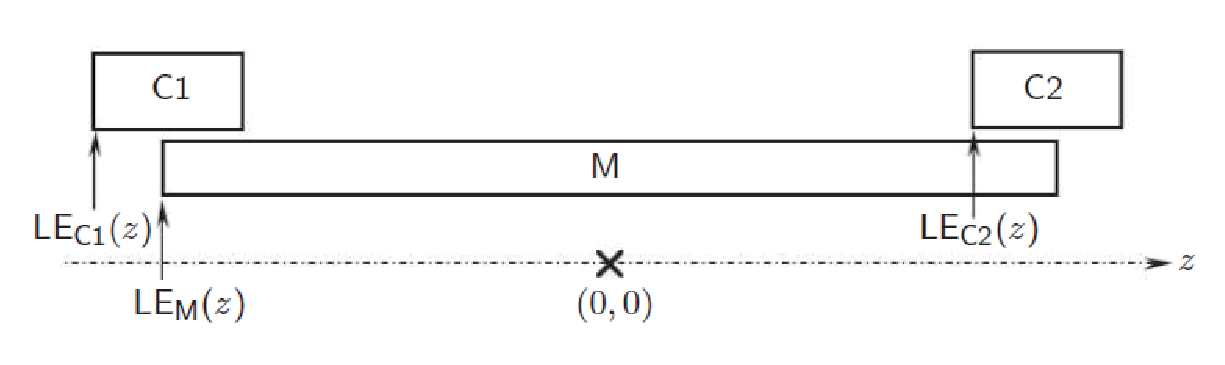
\includegraphics[scale=0.6]{chpt8/figs/fig8.24.eps}
	\caption{Schematic drawing of a magnet comprised of three solenoids}
\end{figure}


\begin{figure}
	\centering
	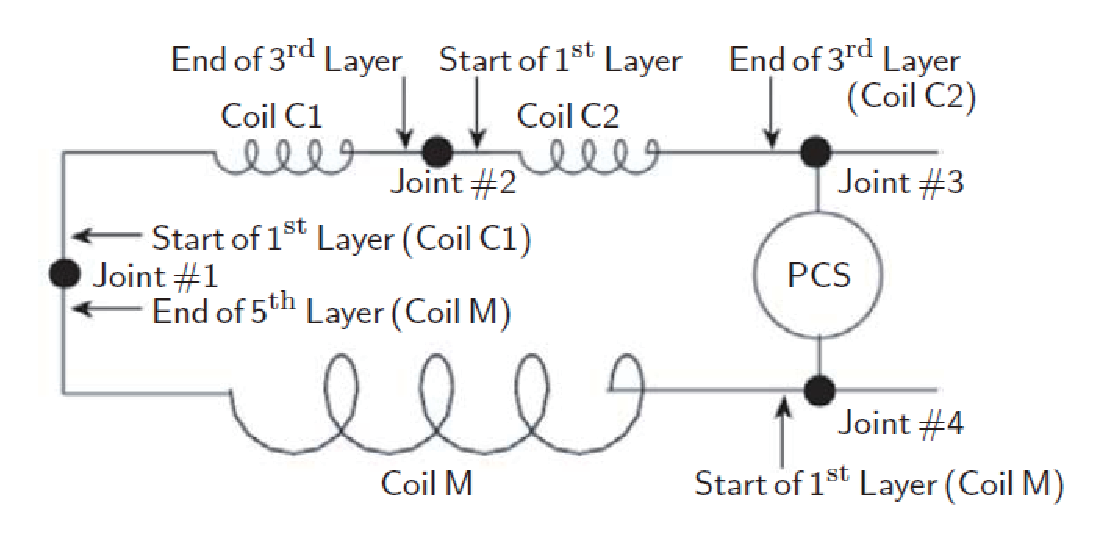
\includegraphics[scale=0.6]{chpt8/figs/fig8.25.eps}
	\caption{Schematic drawing of a 3-coil arrangement, shunted by PCS for persistent}
\end{figure}




\begin{equation}% page528 8.9c
\int_{T_i}^{T_f}\frac{C_m(T)}{\rho_m(T)}dT=\left(\frac{A_m}{A_{cd}}\right)J_{m_o}^{2}\tau_{ah}
\end{equation}
\begin{equation}% page528 6.33
R_{mz}=\sqrt{\frac{3k_{wd}(T_c-T_{op})}{\rho_mJ_{m}^{2}}}
\end{equation}
\begin{equation}% 8.83a
V_M(t)=V_r(t)+(L_M+M_{MC1}+M_{MC2})\frac{dI_{op}(t)}{dt}
\end{equation}
\begin{equation}% 8.83b
V_{C1}(t)=(L_{C1}+M_{C1M}+M_{C1C2})\frac{dI_{op}}{dt}=V_{C2}(t)=-\frac{1}{2}V_M(t)
\end{equation}
\begin{equation}% 8.83c
V_M(t)+V_{C1}(t)+V_{C2}(t)=0
\end{equation}



\subsection{问题8.6:NMR磁体的被动保护}


\begin{figure}
	\centering
	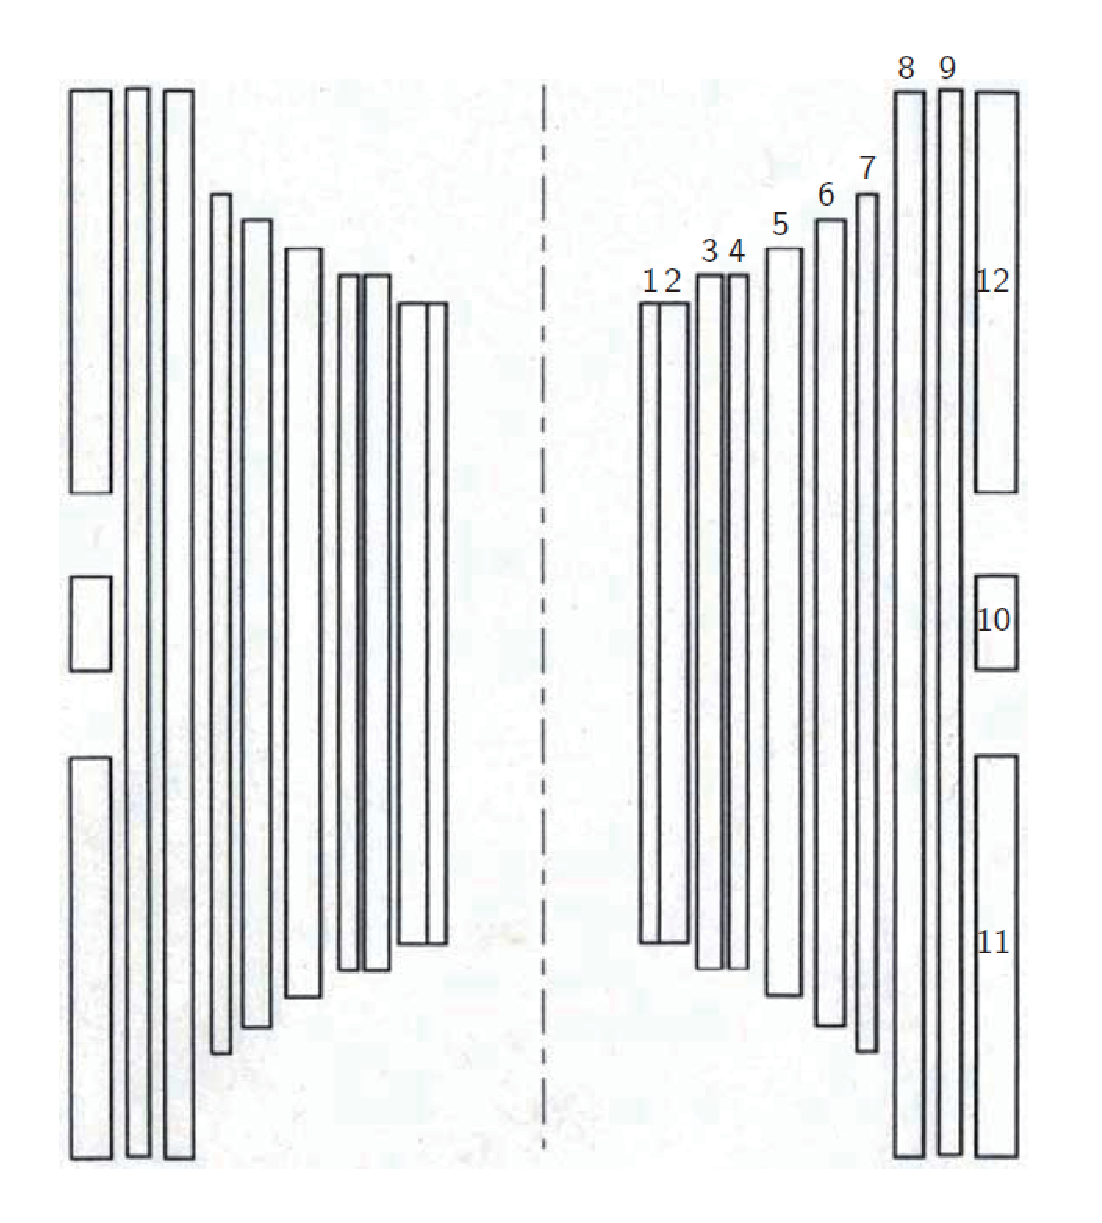
\includegraphics[scale=0.6]{chpt8/figs/fig8.26.eps}
	\caption{Drawing showing the locations of 12 coils in }
\end{figure}


\begin{figure}
	\centering
	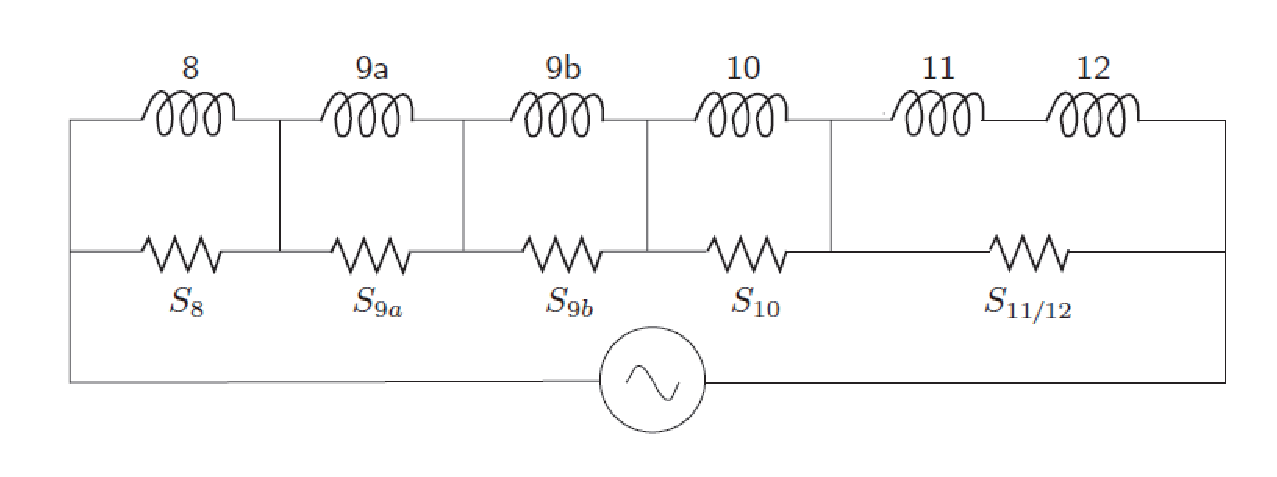
\includegraphics[scale=0.6]{chpt8/figs/fig8.27.eps}
	\caption{Circuit for the NbTi coils}
\end{figure}


\begin{figure}
	\centering
	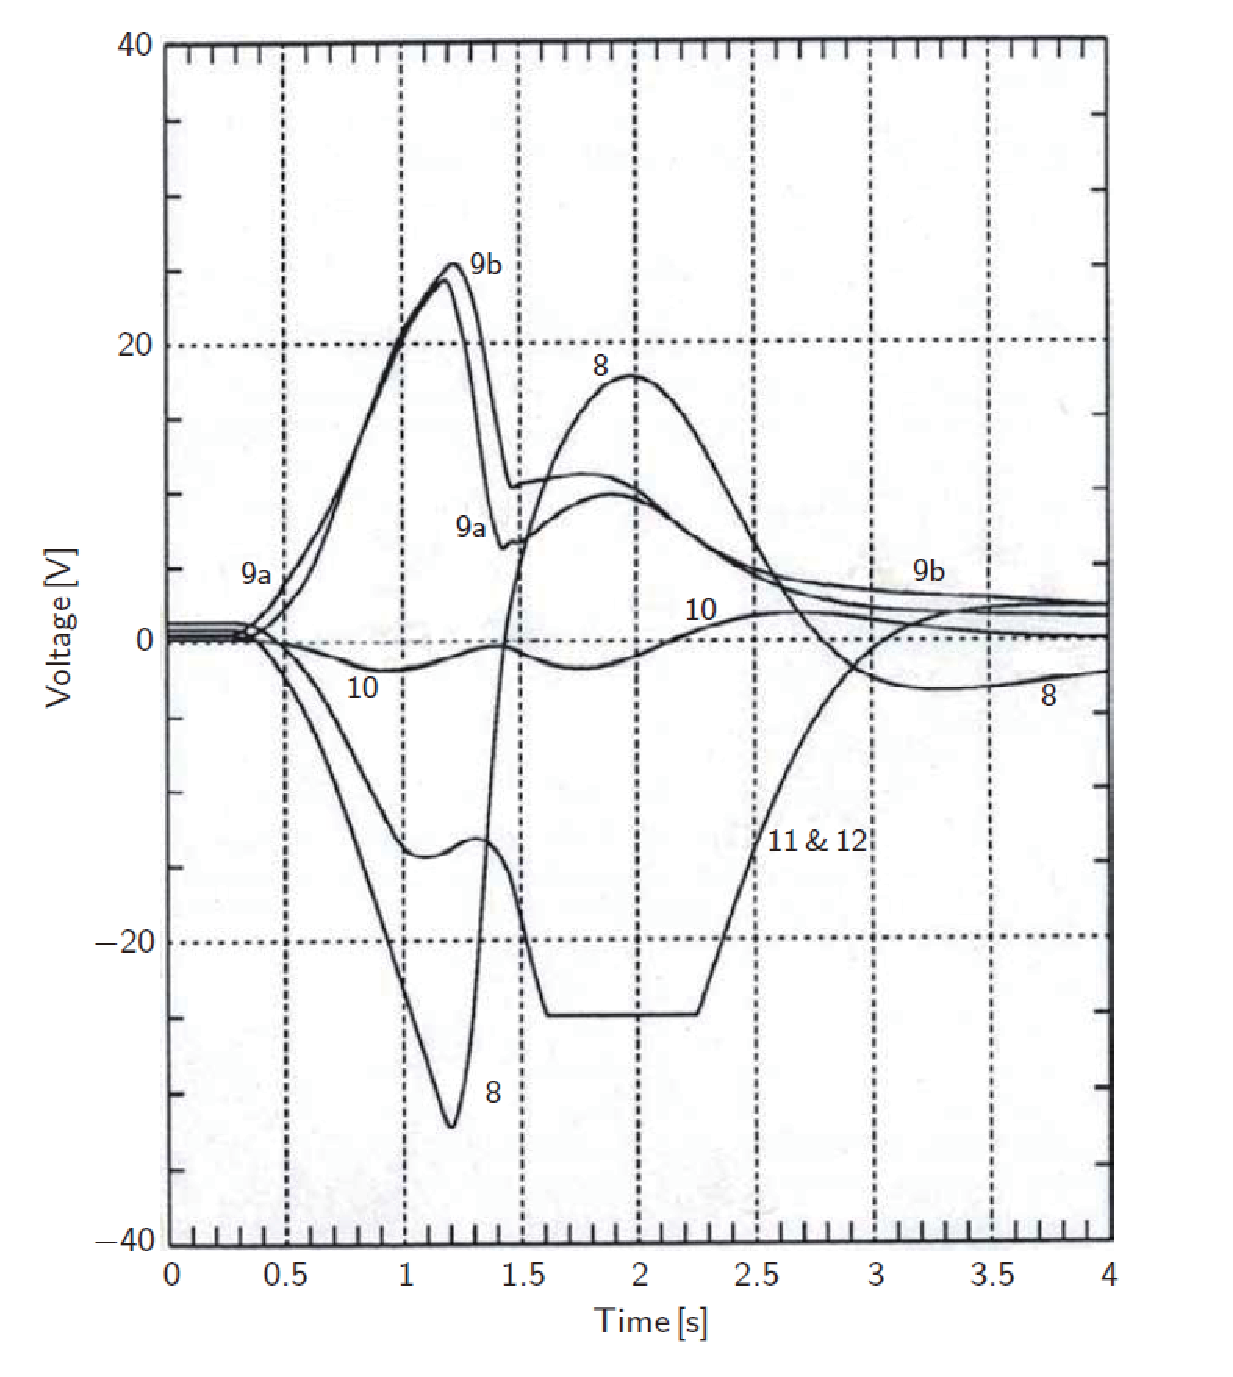
\includegraphics[scale=0.6]{chpt8/figs/fig8.28.eps}
	\caption{Voltage traces recorded acro}
\end{figure}


\begin{figure}
	\centering
	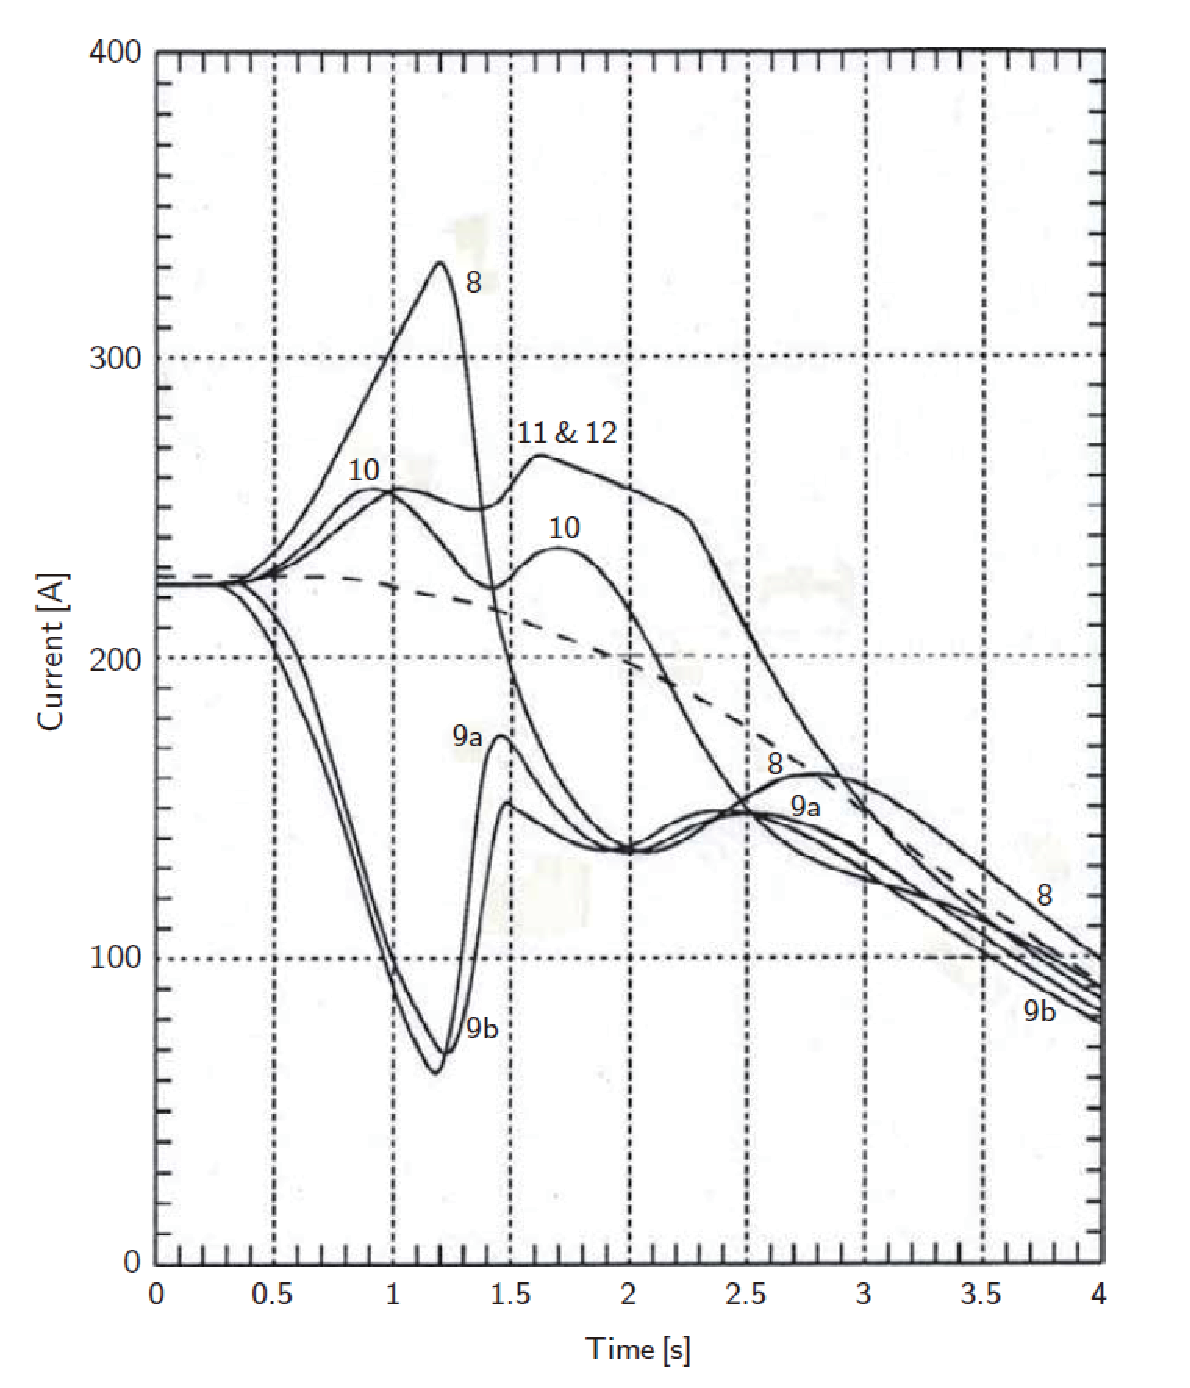
\includegraphics[scale=0.6]{chpt8/figs/fig8.29.eps}
	\caption{Current traces through Coils 8, 9a, 9b, 10, and 11/12 corresponding}
\end{figure}



\begin{equation}% 8.84a
I_8=I_0-\frac{V_8}{S_8}
\end{equation}
\begin{equation}% 8.84b
I_{9a}=I_0-\frac{V_{9a}}{S_{9a}}
\end{equation}
\begin{equation}% 8.84c
I_{9b}=I_0-\frac{V_{9b}}{S_{9b}}
\end{equation}
\begin{equation}% 8.84d
I_{10}=I_0-\frac{V_{10}}{S_{10}}
\end{equation}
\begin{equation}% 8.84e
I_{11/12}=I_0\frac{V_{11/12}}{S_{11/12}}
\end{equation}


\subsubsection{问题8.6之解}

\begin{equation}% page535 8.84a
I_8=I_0-I_{r8}  
=I_0-\frac{V_8}{S_8}
\end{equation}
\begin{equation}% page535 8.84b
I_{9a}=I_8+I_{r8}-I_{r9a}=I_0-\frac{V_8}{S_8}+\frac{V_8}{S_8}-\frac{V_{9a}}{S_{9a}}
=I_0-\frac{V_{9a}}{S_{9a}}
\end{equation}
\begin{equation}% page535 8.84c
I_{9b}=I_{9a}+\frac{V_{9a}}{S_{9a}}-\frac{V_{9b}}{S_{9b}}=I_0-\frac{V_{9a}}{S_{9a}}+\frac{V_{9a}}{S_{9a}}-\frac{V_{9b}}{S_{9b}} 
=I_0\frac{V_{9b}}{S_{9b}}
\end{equation}
\begin{equation}% page535 8.84d
I_{10}=I_{9b}+\frac{V_{9b}}{S_{9b}}-\frac{V_{10}}{S_{10}}=I_0-\frac{V_{9b}}{S_{9b}}+\frac{V_{9b}}{S_{9b}}-\frac{V_{10}}{S_{10}}
=I_0-\frac{V_{10}}{S_{10}}
\end{equation}
\begin{equation}% page535 8.84e
I_{11/12}=I_{10}+\frac{V_{10}}{S_{10}}-\frac{V_{11/12}}{S_{11/12}}=I_0-\frac{V_{10}}{S_{10}}+\frac{V_{10}}{S_{10}}-\frac{V_{11/12}}{S_{11/12}}
=I_0-\frac{V_{11/12}}{S_{11/12}}
\end{equation}
\begin{equation}% page535 S6.1
V_8=V_r\mid_8+L_8\frac{dI_8}{dt}+M_{8,9a}\frac{dI_{9a}}{dt}+M_{8,9b}\frac{dI_{9b}}{dt} 
+M_{8,10}\frac{dI_{10}}{dt}+M_{8,11}\frac{dI_{11}}{dt}+M_{8,12}\frac{dI_{12}}{dt}
\end{equation}
\begin{equation}% page535 S6.2a
V_8\simeq V_r\mid_8+(4.413\ \mathrm{H})(84.5\ \mathrm{A/s})+(2.268\ \mathrm{H})(-154.1\ \mathrm{A/s}) 
+(2.243\ \mathrm{H})(-107.1\ \mathrm{A/s})+(0.715\ \mathrm{H})(41.3\ \mathrm{A/s}) 
+(2.747\ \mathrm{H})(33.6\ \mathrm{A/s})+(2.755\ \mathrm{H})(33.6\ \mathrm{A/s})
\end{equation}
\begin{equation}% page535 S6.2b
V_8=V_r\mid_8+372.9-349.5-240.2+39.4+92.4+92.6 
=V_r\mid_8-2.5\ \mathrm{V}
\end{equation}
\begin{equation}% page536 S6.3a
V_8=V_r\mid_8+(4.413\ \mathrm{H})(147.2\ \mathrm{A/s})+(2.268\ \mathrm{H})(-234.7\ \mathrm{A/s}) 
+(2.243\ \mathrm{H})(-198.1\ \mathrm{A/s})+(0.715\ \mathrm{H})(-44.8\ \mathrm{A/s}) 
+(2.747\ \mathrm{H})(19.3\ \mathrm{A/s})+(2.755\ \mathrm{H})(19.3\ \mathrm{A/s})
\end{equation}
\begin{equation}% page536 S6.3b
V_8=V_r\mid_8+(649.6-532.3-444.3-32.0+53.0+53.2)[\mathrm{V}]
=V_r\mid_8-252.9[\mathrm{V}]
\end{equation}
\begin{equation}% page536 S6.4
P_{mg}=\sum_{n=8}^{12}V_r\mid_n\times I_n
\end{equation}
\begin{equation}% page536 S6.5
P_{mg}\simeq\left(\tilde{V}-\sum_{m,n=8}^{12}L_{m,n}\frac{d\tilde{I}}{dt}\right)\times \tilde{I}
\end{equation}
\begin{equation}% page536 S6.6
P_{mg}\simeq[0-(60.25\ \mathrm{H})(-50\ \mathrm{A/s})](90\ \mathrm{A})\simeq 270,000\ \mathrm{W}
\end{equation}




\subsection{讨论8.7:HTS磁体到底要不要保护?}
\begin{equation}% 8.85a
\$_{T/w}=\$_M+\$_{qp}
\end{equation}
\begin{equation}% 8.85b
\$_{T/wo}=\$_M+P_{dm}(\$_M+\$_{ra})
\end{equation}